\chapter{Performance of a VBS topology identifier}
\label{chap:vbfrnn_results}

This chapter evaluates the VBF-RNN tagger introduced in Section~\ref{sec:vbfrnn} on its ability to isolate the vector boson scattering topology from the inclusive electroweak $VVjj$ production. The three RNN versions of Table~\ref{tab:vbfrnn_versions} are first compared on a common figure of merit, after which the artefacts introduced by the jet multiplicity are discussed, an alternative transformer-based architecture is evaluated and finally the response of the tagger to the different aQGC operator families is studied. The performance reported here motivates the choice of the version~3 score as both a pre-selection requirement and an input feature to the aQGC discriminant of Chapter~\ref{chap:analysismethods}.

\section{Evaluation sample and figure of merit}
\label{sec:vbfrnn_eval}

The tagger is evaluated on the statistically independent validation sample of electroweak $VVjj$ events described in Section~\ref{sec:vbfrnn}, using the truth-level VBS / non-VBS labels obtained from the boson- and tagging-jet matching procedure. The combined $WW$, $WZ$ and $ZZ$ final states are merged into a single sample, so that the quoted performance reflects the inclusive diboson channel relevant to the fully hadronic analysis, with consistent behaviour across the individual channels.

Because the tagger output is a continuous score $s\in[0,1]$, its discriminating power is quantified with the receiver operating characteristic (ROC) curve. For a given threshold $s_{\mathrm{cut}}$, events with $s>s_{\mathrm{cut}}$ are tagged as VBS. The true-positive rate (the VBS efficiency, or VBS positive rate) is the fraction of true VBS events that are tagged, while the false-positive rate (the non-VBS positive rate) is the fraction of non-VBS EWK events that are also tagged. Sweeping $s_{\mathrm{cut}}$ from $1$ to $0$ traces out the ROC curve in the (false-positive rate, true-positive rate) plane. A perfect classifier reaches the top-left corner, whereas a random classifier lies on the diagonal. The area under this curve (AUC) condenses the curve into a single scalar: it equals the probability that a randomly chosen VBS event is assigned a higher score than a randomly chosen non-VBS event, so that $\mathrm{AUC}=1$ is perfect separation and $\mathrm{AUC}=0.5$ is no separation. The AUC is used throughout this chapter as the primary figure of merit.

\section{Performance comparison of the RNN versions}
\label{sec:vbfrnn_perf}

The three RNN versions are compared on the combined diboson validation sample in Figure~\ref{fig:vbfrnn_roc} and summarised in Table~\ref{tab:vbfrnn_auc}. Version~1, trained to separate resonant VBF from gluon-fusion production using only the four leading tagging jets, generalises poorly to the VBS versus non-VBS EWK task it is applied to here, reaching an AUC of only $0.629$ and lying close to the diagonal. Retraining the identical four-jet architecture directly on the VBS versus non-VBS EWK objective (version~2) raises the AUC substantially to $0.760$, confirming that the relevant topological information is accessible from the tagging-jet kinematics once the network is optimised for the correct target. Extending the input to six jets by adding the two large-$R$ signal jets (version~3) improves the AUC further to $0.801$.

The motivation for adding the signal jets is shown in Figure~\ref{fig:vbfrnn_sigjet}: the dijet invariant mass of the two large-$R$ signal jets retains discriminating power between the VBS and non-VBS EWK topologies that is not captured by the tagging jets alone. Exploiting this information yields a relative AUC improvement of $+5.4\%$ from version~2 to version~3. The corresponding score distributions, shown in Figure~\ref{fig:vbfrnn_scores}, illustrate the effect directly: for the four-jet tagger the VBS and non-VBS EWK distributions overlap substantially, whereas for the six-jet tagger the non-VBS EWK events are pushed towards low scores and the VBS events towards high scores, giving a markedly cleaner separation. Version~3 is therefore adopted as the baseline tagger for the remainder of the analysis.

\begin{table}[h]
\centering
\caption{Discrimination performance of the three VBF-RNN versions on the combined $WW+WZ+ZZ$ EWK validation sample, quantified by the AUC for separating VBS from non-VBS EWK events. The relative improvement is given with respect to the preceding configuration.}
\label{tab:vbfrnn_auc}
\begin{tabular}{llcc}
\toprule
Version & Configuration & AUC & Relative improvement \\
\midrule
v1 & 4 jets, VBF vs.\ ggF         & 0.629 & --- \\
v2 & 4 jets, VBS vs.\ non-VBS EWK & 0.760 & $+20.8\%$ \\
v3 & 6 jets, VBS vs.\ non-VBS EWK & 0.801 & $+5.4\%$ \\
\bottomrule
\end{tabular}
\end{table}

\begin{figure}[h]
\centering
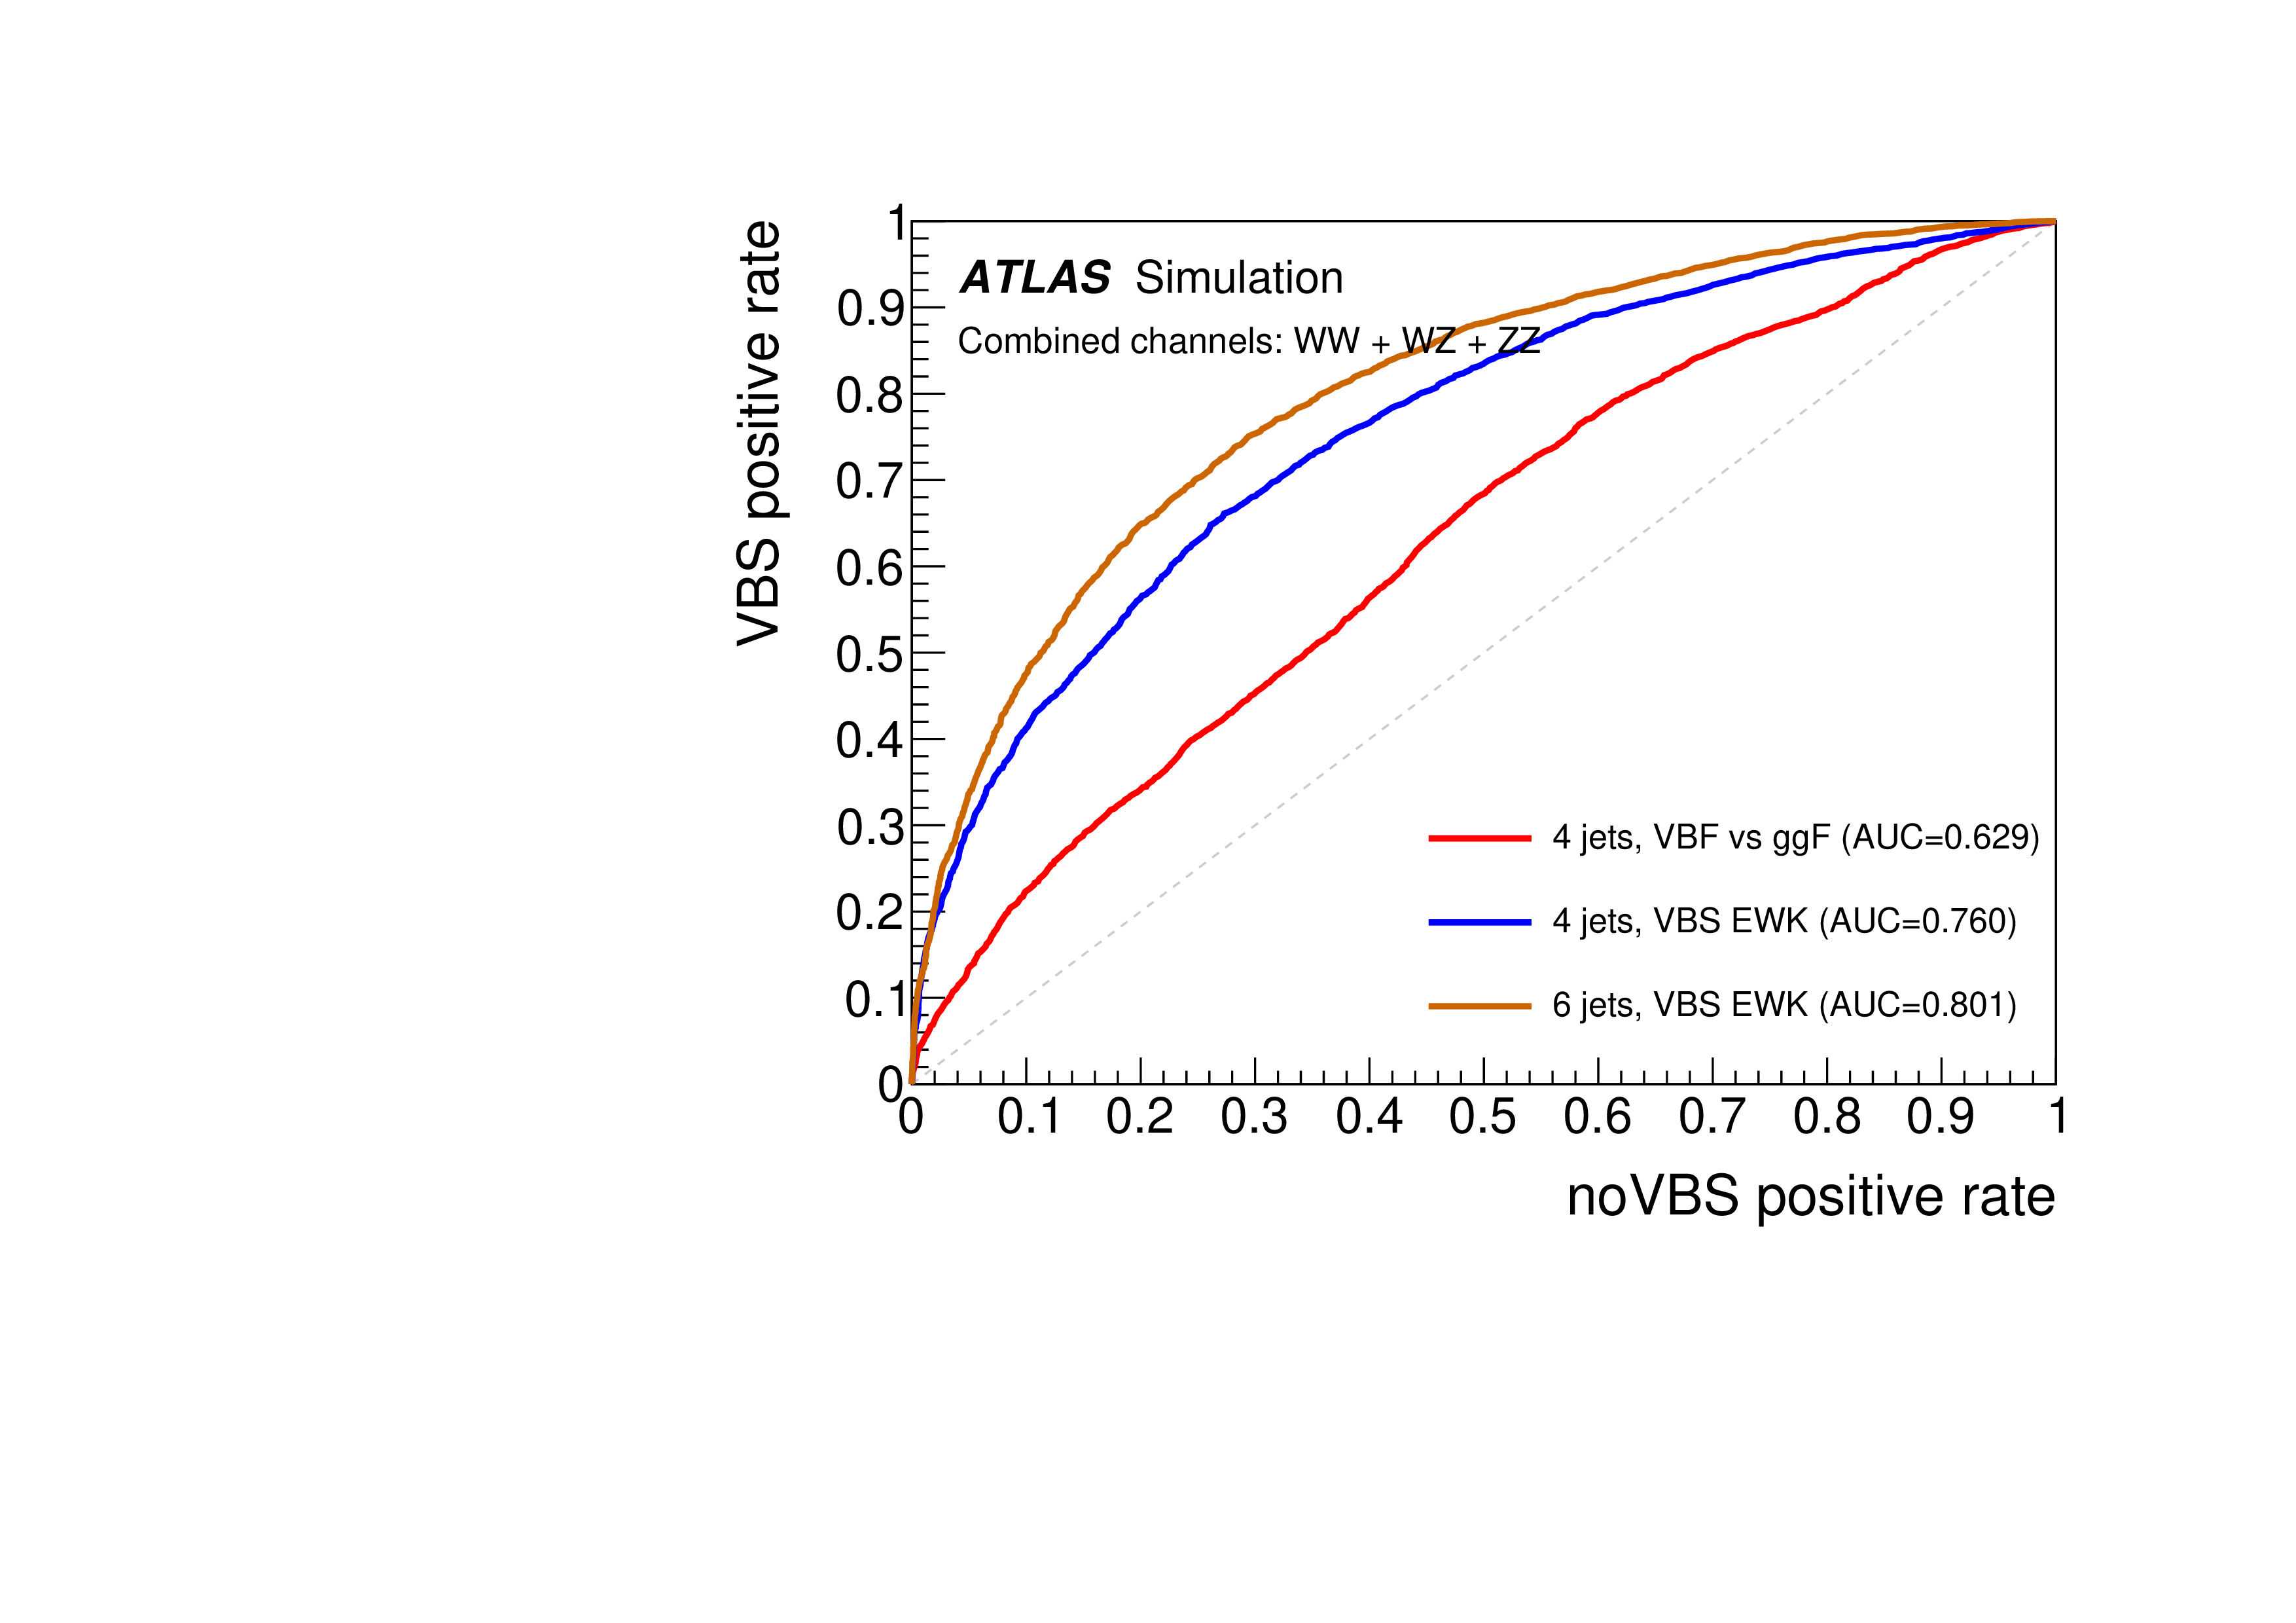
\includegraphics[width=0.7\textwidth]{figures/vbfrnn_roc_versions.png}
\caption{ROC curves for the three VBF-RNN versions evaluated on the combined $WW+WZ+ZZ$ EWK validation sample, separating VBS from non-VBS EWK events. The vertical axis is the VBS positive rate (true-positive rate) and the horizontal axis the non-VBS positive rate (false-positive rate). Curves are shown for version~1 (4 jets, VBF vs.\ ggF, $\mathrm{AUC}=0.629$), version~2 (4 jets, VBS vs.\ non-VBS EWK, $\mathrm{AUC}=0.760$) and version~3 (6 jets, VBS vs.\ non-VBS EWK, $\mathrm{AUC}=0.801$). The dashed diagonal indicates a random classifier.}
\label{fig:vbfrnn_roc}
\end{figure}

\begin{figure}[h]
\centering
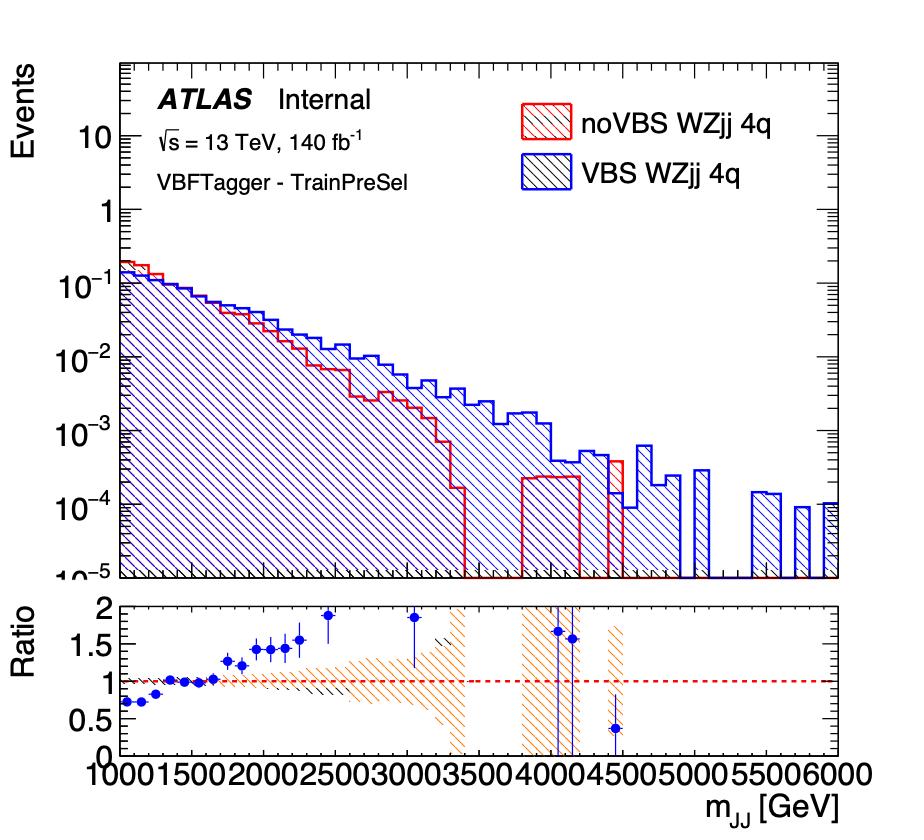
\includegraphics[width=0.6\textwidth]{figures/vbfrnn_sigjet_mjj.png}
\caption{Normalised distribution of the dijet invariant mass of the two large-$R$ signal jets at the training pre-selection, for VBS (blue) and non-VBS EWK (red) $WZjj\to 4q$ events. The difference between the two distributions, quantified by the ratio panel, demonstrates the additional discriminating information that motivates including the signal jets in version~3 of the tagger.}
\label{fig:vbfrnn_sigjet}
\end{figure}

\begin{figure}[h]
\centering
\begin{subfigure}[b]{0.48\textwidth}
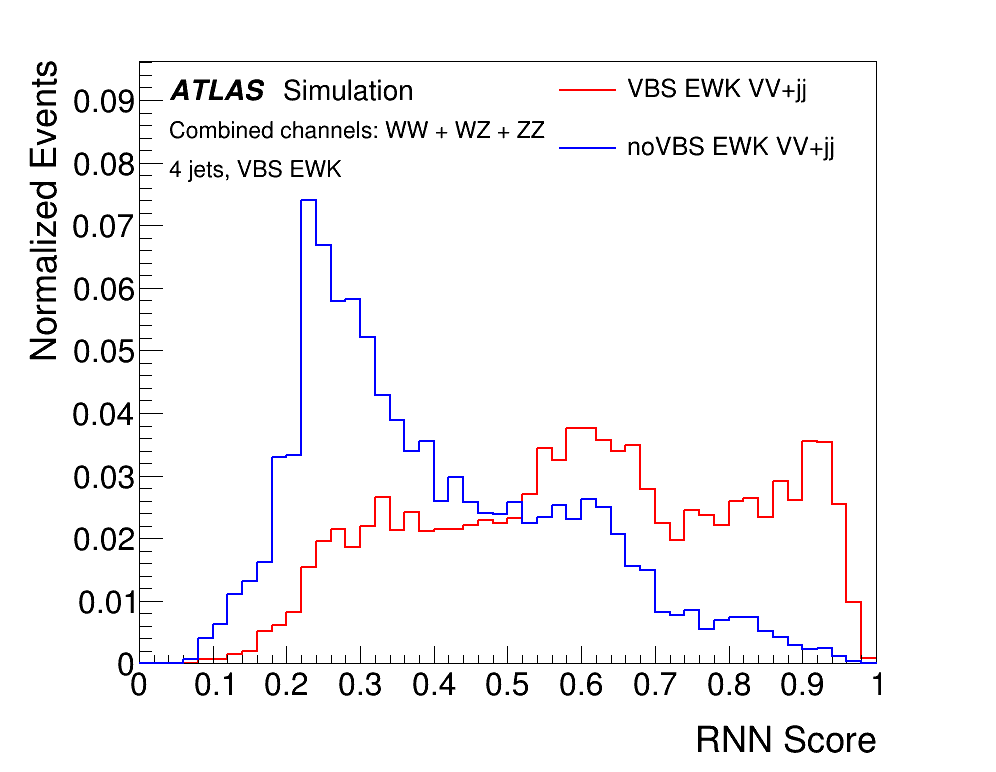
\includegraphics[width=\textwidth]{figures/vbfrnn_score_v2.png}
\caption{Version~2 (4 jets)}
\end{subfigure}
\hfill
\begin{subfigure}[b]{0.48\textwidth}
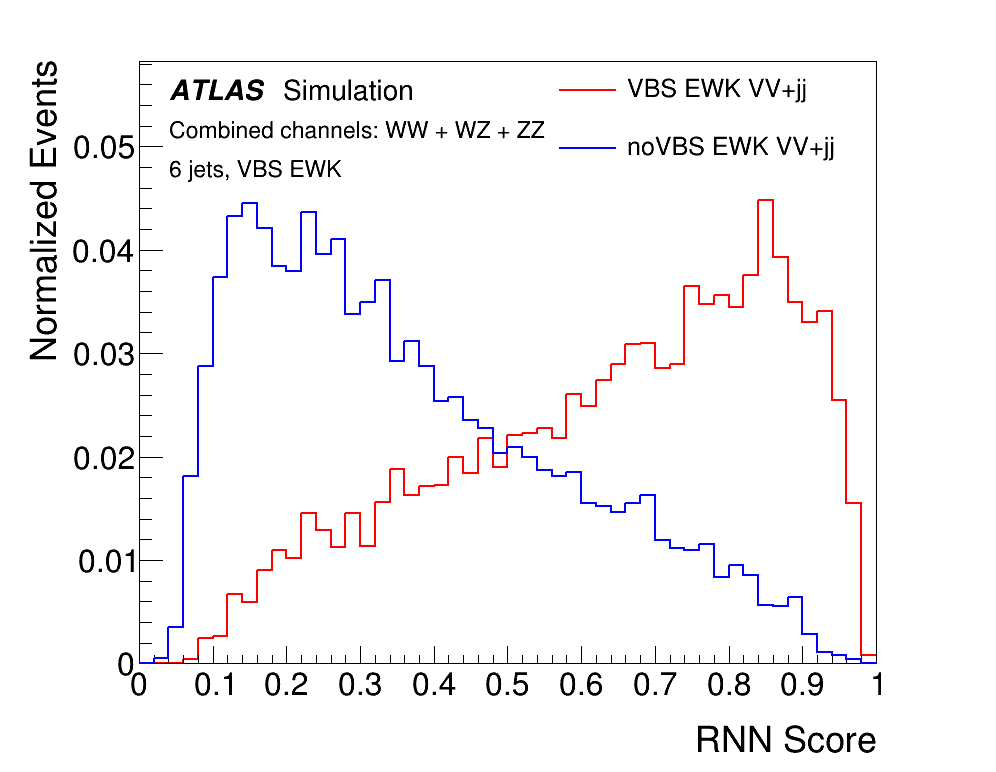
\includegraphics[width=\textwidth]{figures/vbfrnn_score_v3.png}
\caption{Version~3 (6 jets)}
\end{subfigure}
\caption{VBF-RNN score distributions for VBS (blue) and non-VBS EWK (red) events, for the four-jet version~2 (left) and the six-jet version~3 (right) tagger. Including the signal jets sharpens the separation, pushing non-VBS EWK events to low scores and VBS events to high scores. The residual structure near $s\approx0.9$ in the four-jet distribution is discussed in Section~\ref{sec:vbfrnn_multiplicity}.}
\label{fig:vbfrnn_scores}
\end{figure}

\section{Effect of the input jet multiplicity}
\label{sec:vbfrnn_multiplicity}

The version~2 score distributions in Figure~\ref{fig:vbfrnn_scores} exhibit a localised artefact, a sharp dip in the distribution near high score values, that is absent in the cleaner version~3 distributions. This structure is traced to the number of jets actually available as input to the RNN. Figure~\ref{fig:vbfrnn_njets} shows the RNN score as a function of the number of input jets for the four-jet EWK model. Events in which only a single jet is passed to the network, which occurs when the remaining jets fall outside the detector acceptance or fail reconstruction, are structurally unable to be assigned high scores, since the topological correlations the network relies on require at least two jets. These low-multiplicity events accumulate at intermediate scores and are responsible for the discontinuities seen in the version~2 distribution. Splitting the score distribution into events with exactly one input jet and events with two or more, shown for each aQGC operator family in Figure~\ref{fig:vbfrnn_njets_split}, confirms that the artefact originates entirely from the single-jet population. Adding the two large-$R$ signal jets in version~3 guarantees a minimum input multiplicity for every event, which removes the artefact and is a further reason to prefer version~3.

\begin{figure}[h]
\centering
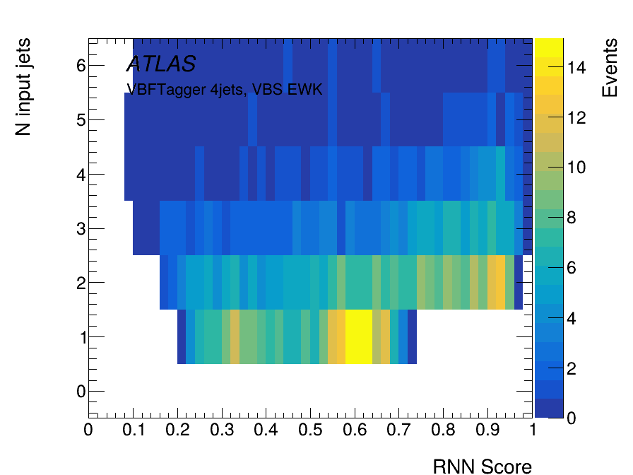
\includegraphics[width=0.55\textwidth]{figures/vbfrnn_njets_vs_score.png}
\caption{Two-dimensional distribution of the number of input jets versus the VBF-RNN score for the four-jet EWK (version~2) model. Single-jet events fail to be assigned high scores and produce the artefacts visible in the version~2 score distribution of Figure~\ref{fig:vbfrnn_scores}.}
\label{fig:vbfrnn_njets}
\end{figure}

\begin{figure}[h]
\centering
\begin{subfigure}[b]{0.32\textwidth}
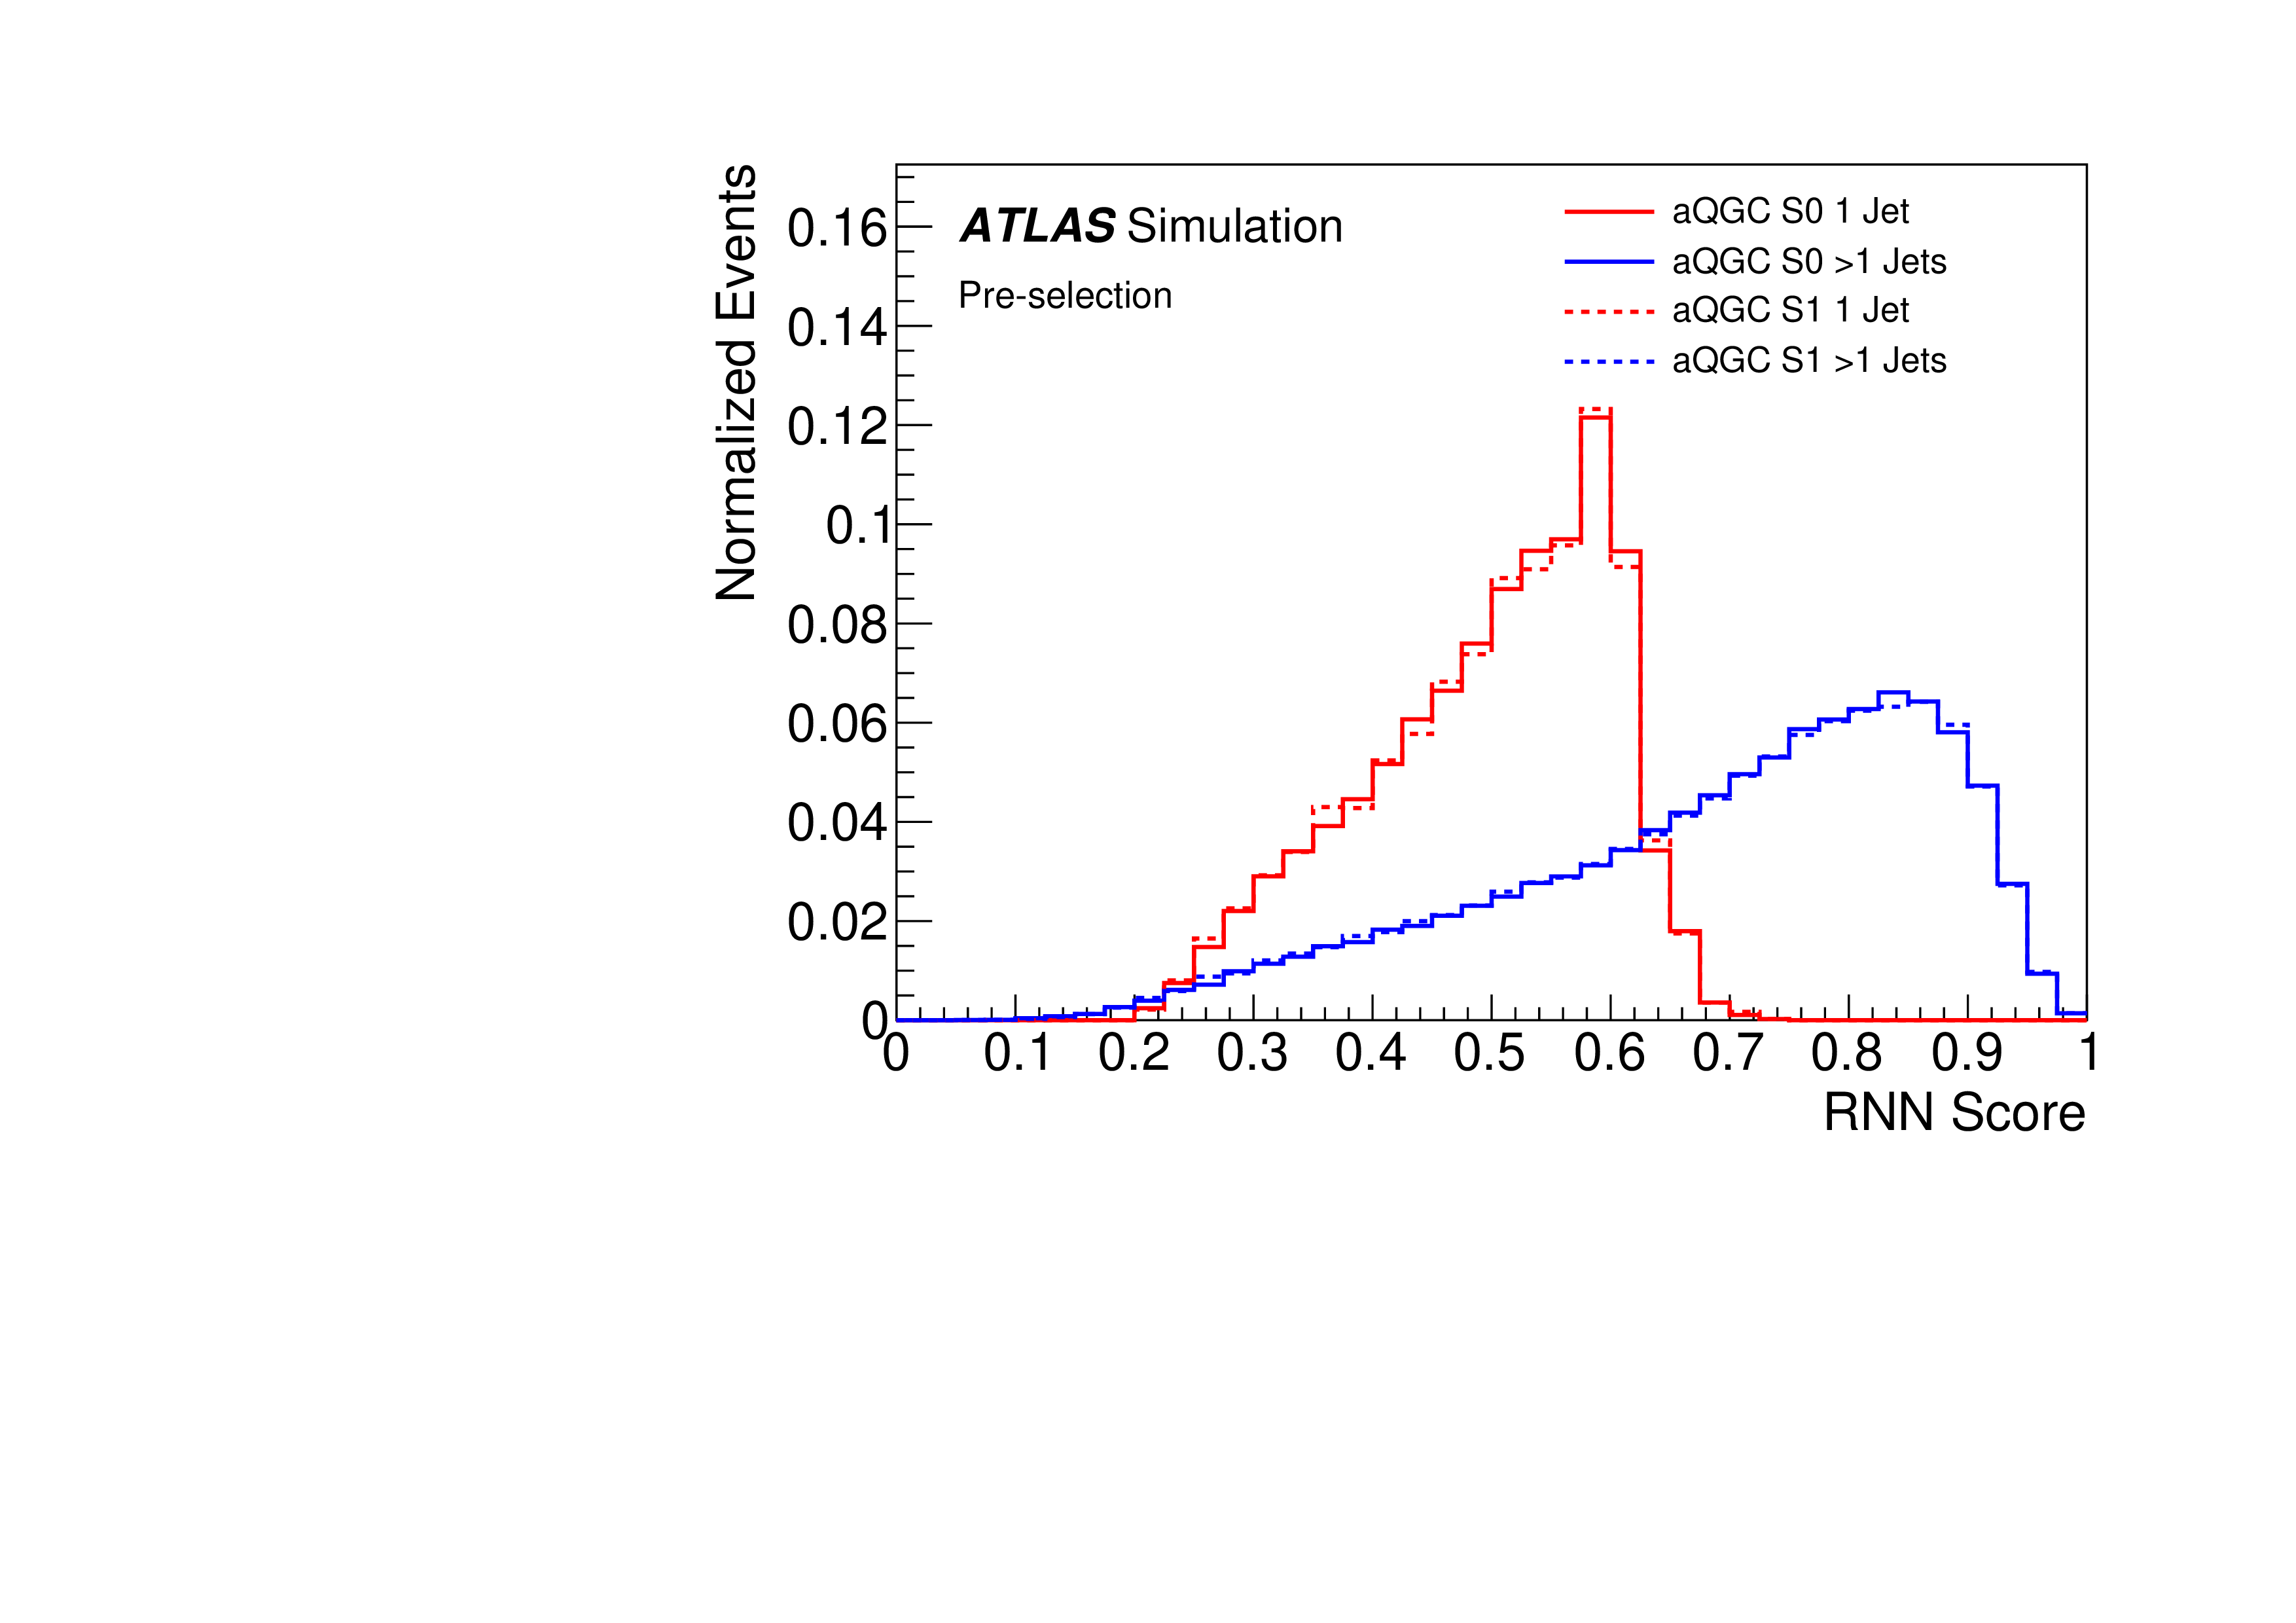
\includegraphics[width=\textwidth]{figures/vbfrnn_aqgc_v2_S_njets.png}
\caption{Scalar}
\end{subfigure}
\begin{subfigure}[b]{0.32\textwidth}
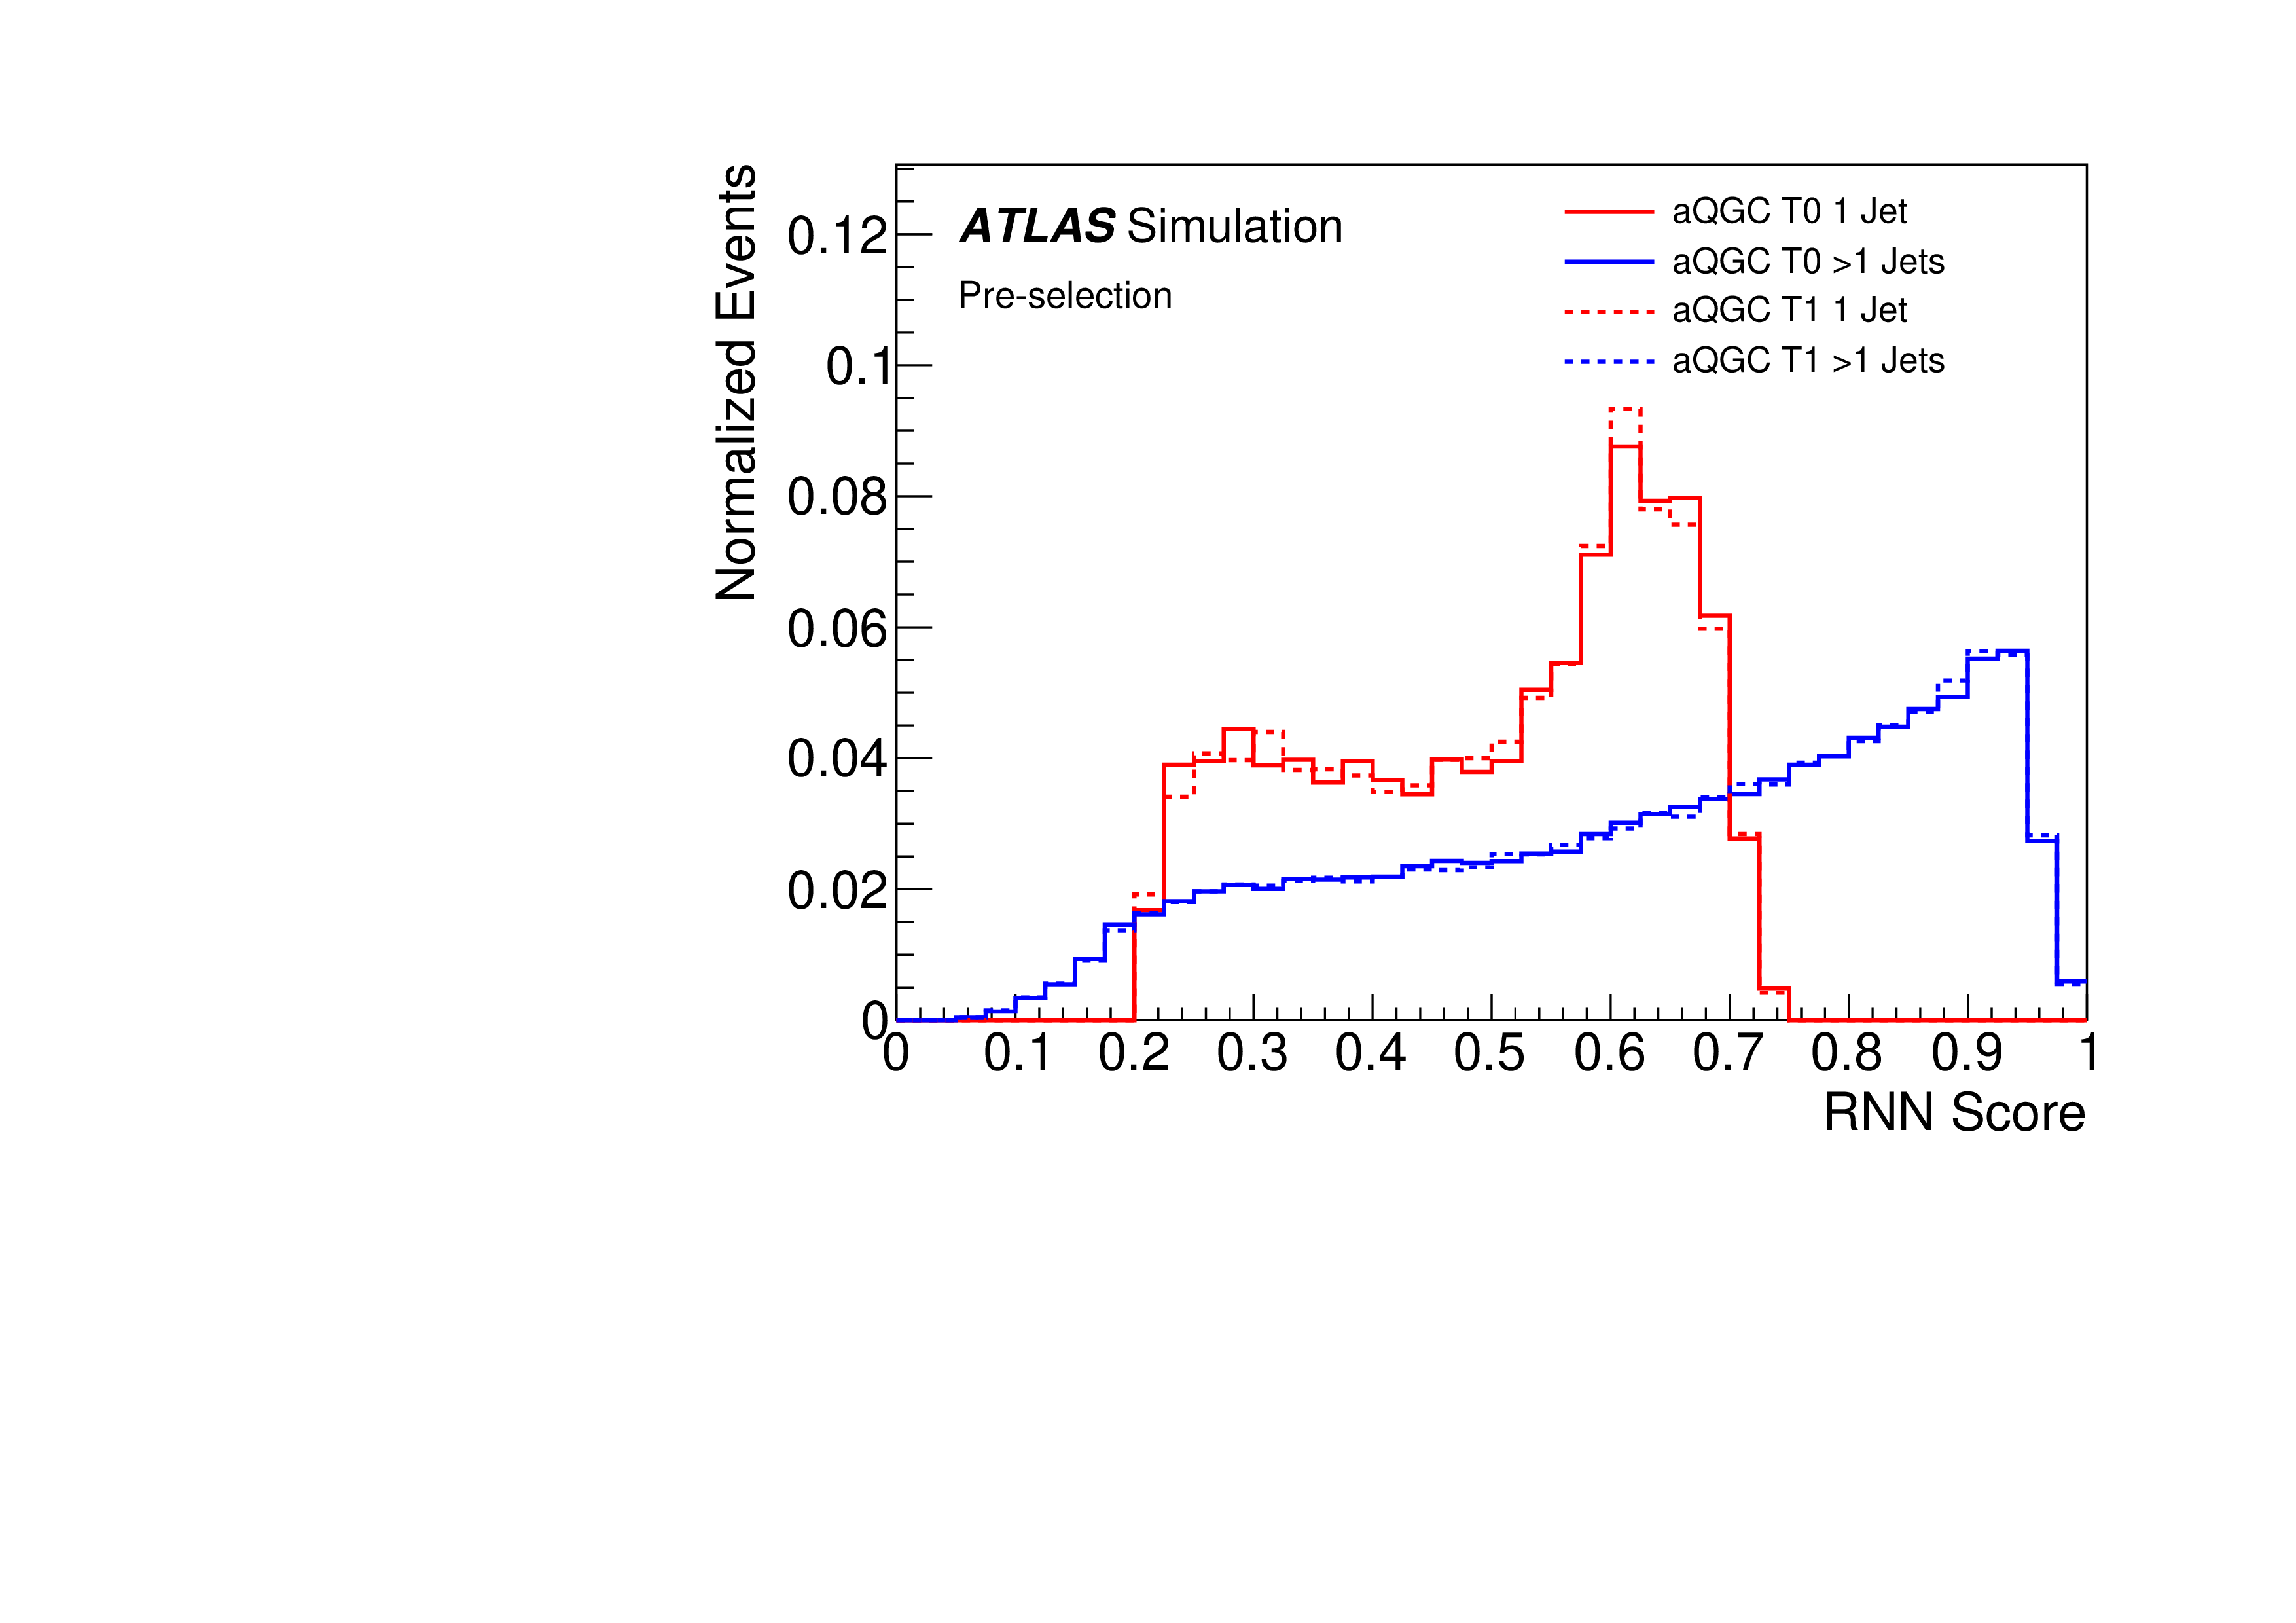
\includegraphics[width=\textwidth]{figures/vbfrnn_aqgc_v2_T_njets.png}
\caption{Tensor}
\end{subfigure}
\begin{subfigure}[b]{0.32\textwidth}
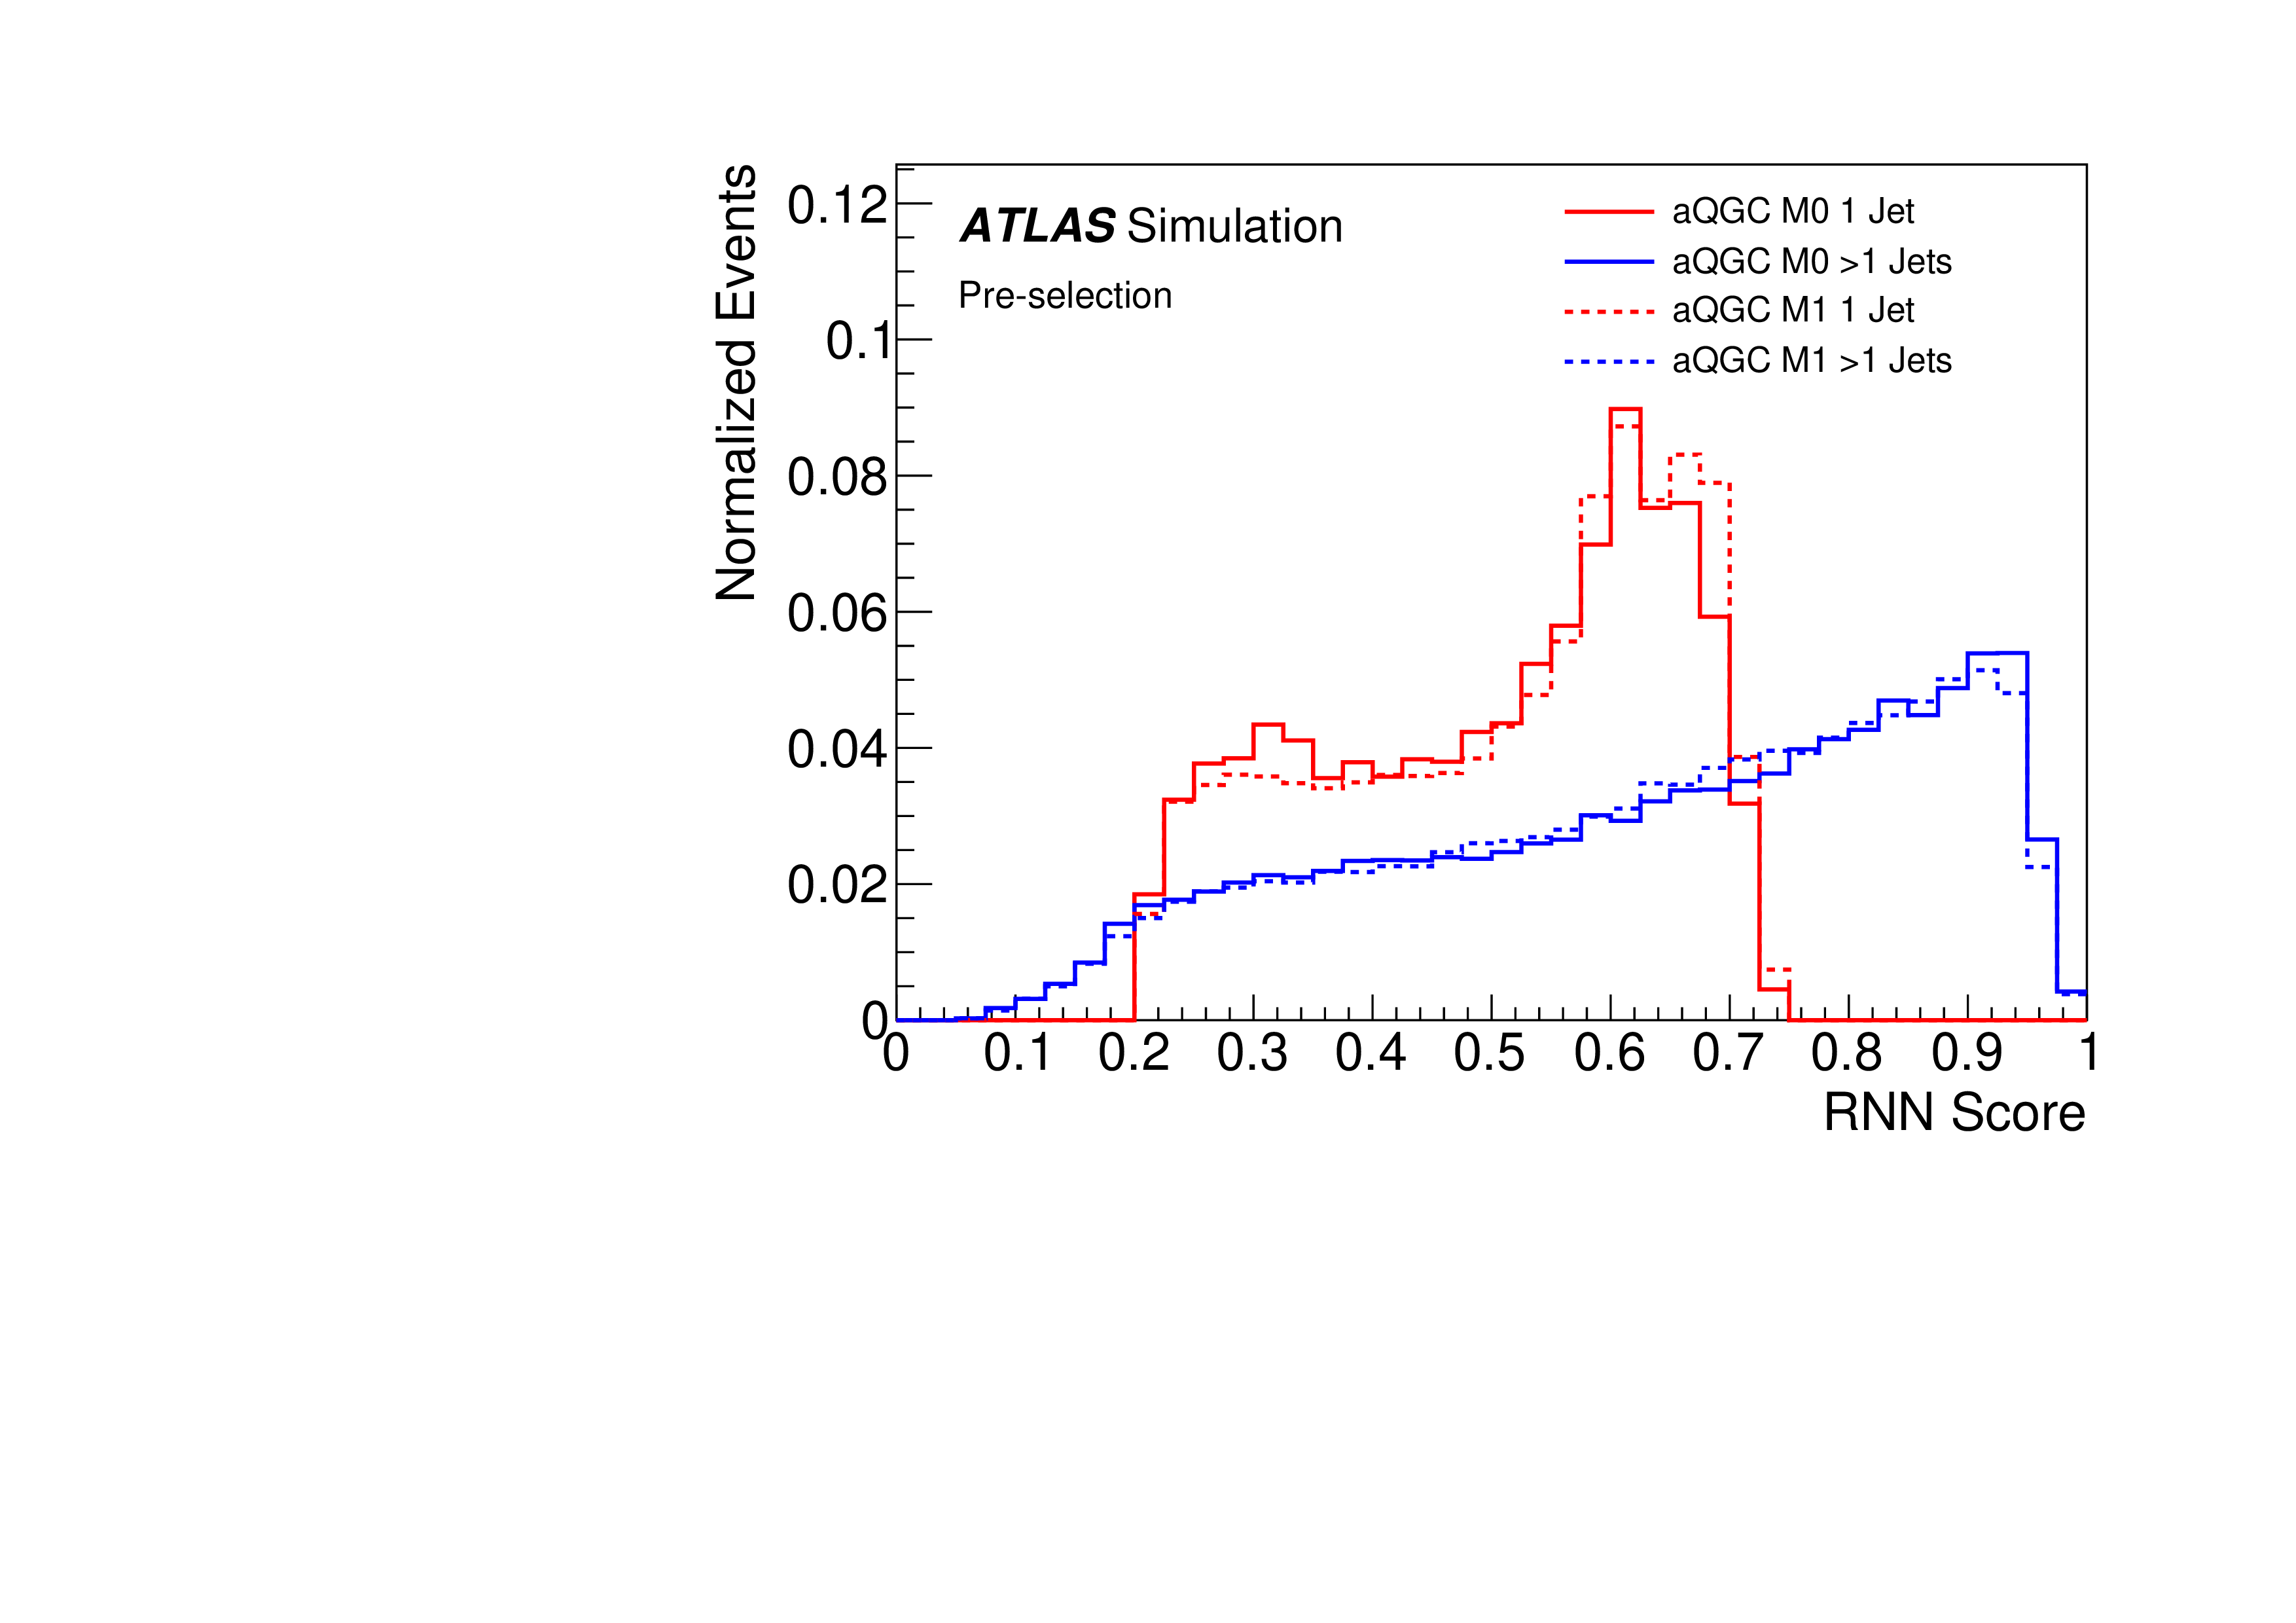
\includegraphics[width=\textwidth]{figures/vbfrnn_aqgc_v2_M_njets.png}
\caption{Mixed}
\end{subfigure}
\caption{Version~2 (4 jets) VBF-RNN score for events with exactly one input jet (red) and with two or more input jets (black), shown separately for representative scalar, tensor and mixed aQGC operators. Across all three families the single-jet population fails to reach high scores, confirming that the artefact in the version~2 score distribution originates entirely from low-multiplicity events.}
\label{fig:vbfrnn_njets_split}
\end{figure}

\section{Transformer architecture}
\label{sec:vbfrnn_transformer}

The recurrent architecture propagates information sequentially through the jet collection and may lose distant context for longer input sequences. A transformer encoder, which computes pairwise interactions between all input jets simultaneously through the self-attention mechanism described in Chapter~\ref{chap:ml}, was trained on the identical six-jet input and VBS versus non-VBS EWK target as version~3 to test whether the global attention structure offers a tangible benefit.

Adding the transformer curve to the ROC comparison, shown in Figure~\ref{fig:vbfrnn_roc_transformer} and summarised in Table~\ref{tab:vbfrnn_transformer_auc}, yields an AUC of $0.806$, a marginal improvement of $+0.6\%$ over the version~3 RNN ($0.801$). The two curves are essentially indistinguishable and, in particular, the transformer offers no gain in the high-VBS-efficiency regime relevant to the analysis. Given the negligible performance difference and the higher computational cost of the attention mechanism for the short jet sequences used here, the recurrent version~3 tagger is retained as the baseline.

\begin{table}[h]
\centering
\caption{AUC of the recurrent version~3 tagger and the transformer encoder trained on the identical six-jet input and VBS versus non-VBS EWK target, with the relative improvement of the transformer over the RNN.}
\label{tab:vbfrnn_transformer_auc}
\begin{tabular}{lcc}
\toprule
Model & AUC & Relative improvement \\
\midrule
RNN v3 (6 jets)      & 0.801 & --- \\
Transformer (6 jets) & 0.806 & $+0.6\%$ \\
\bottomrule
\end{tabular}
\end{table}

\begin{figure}[h]
\centering
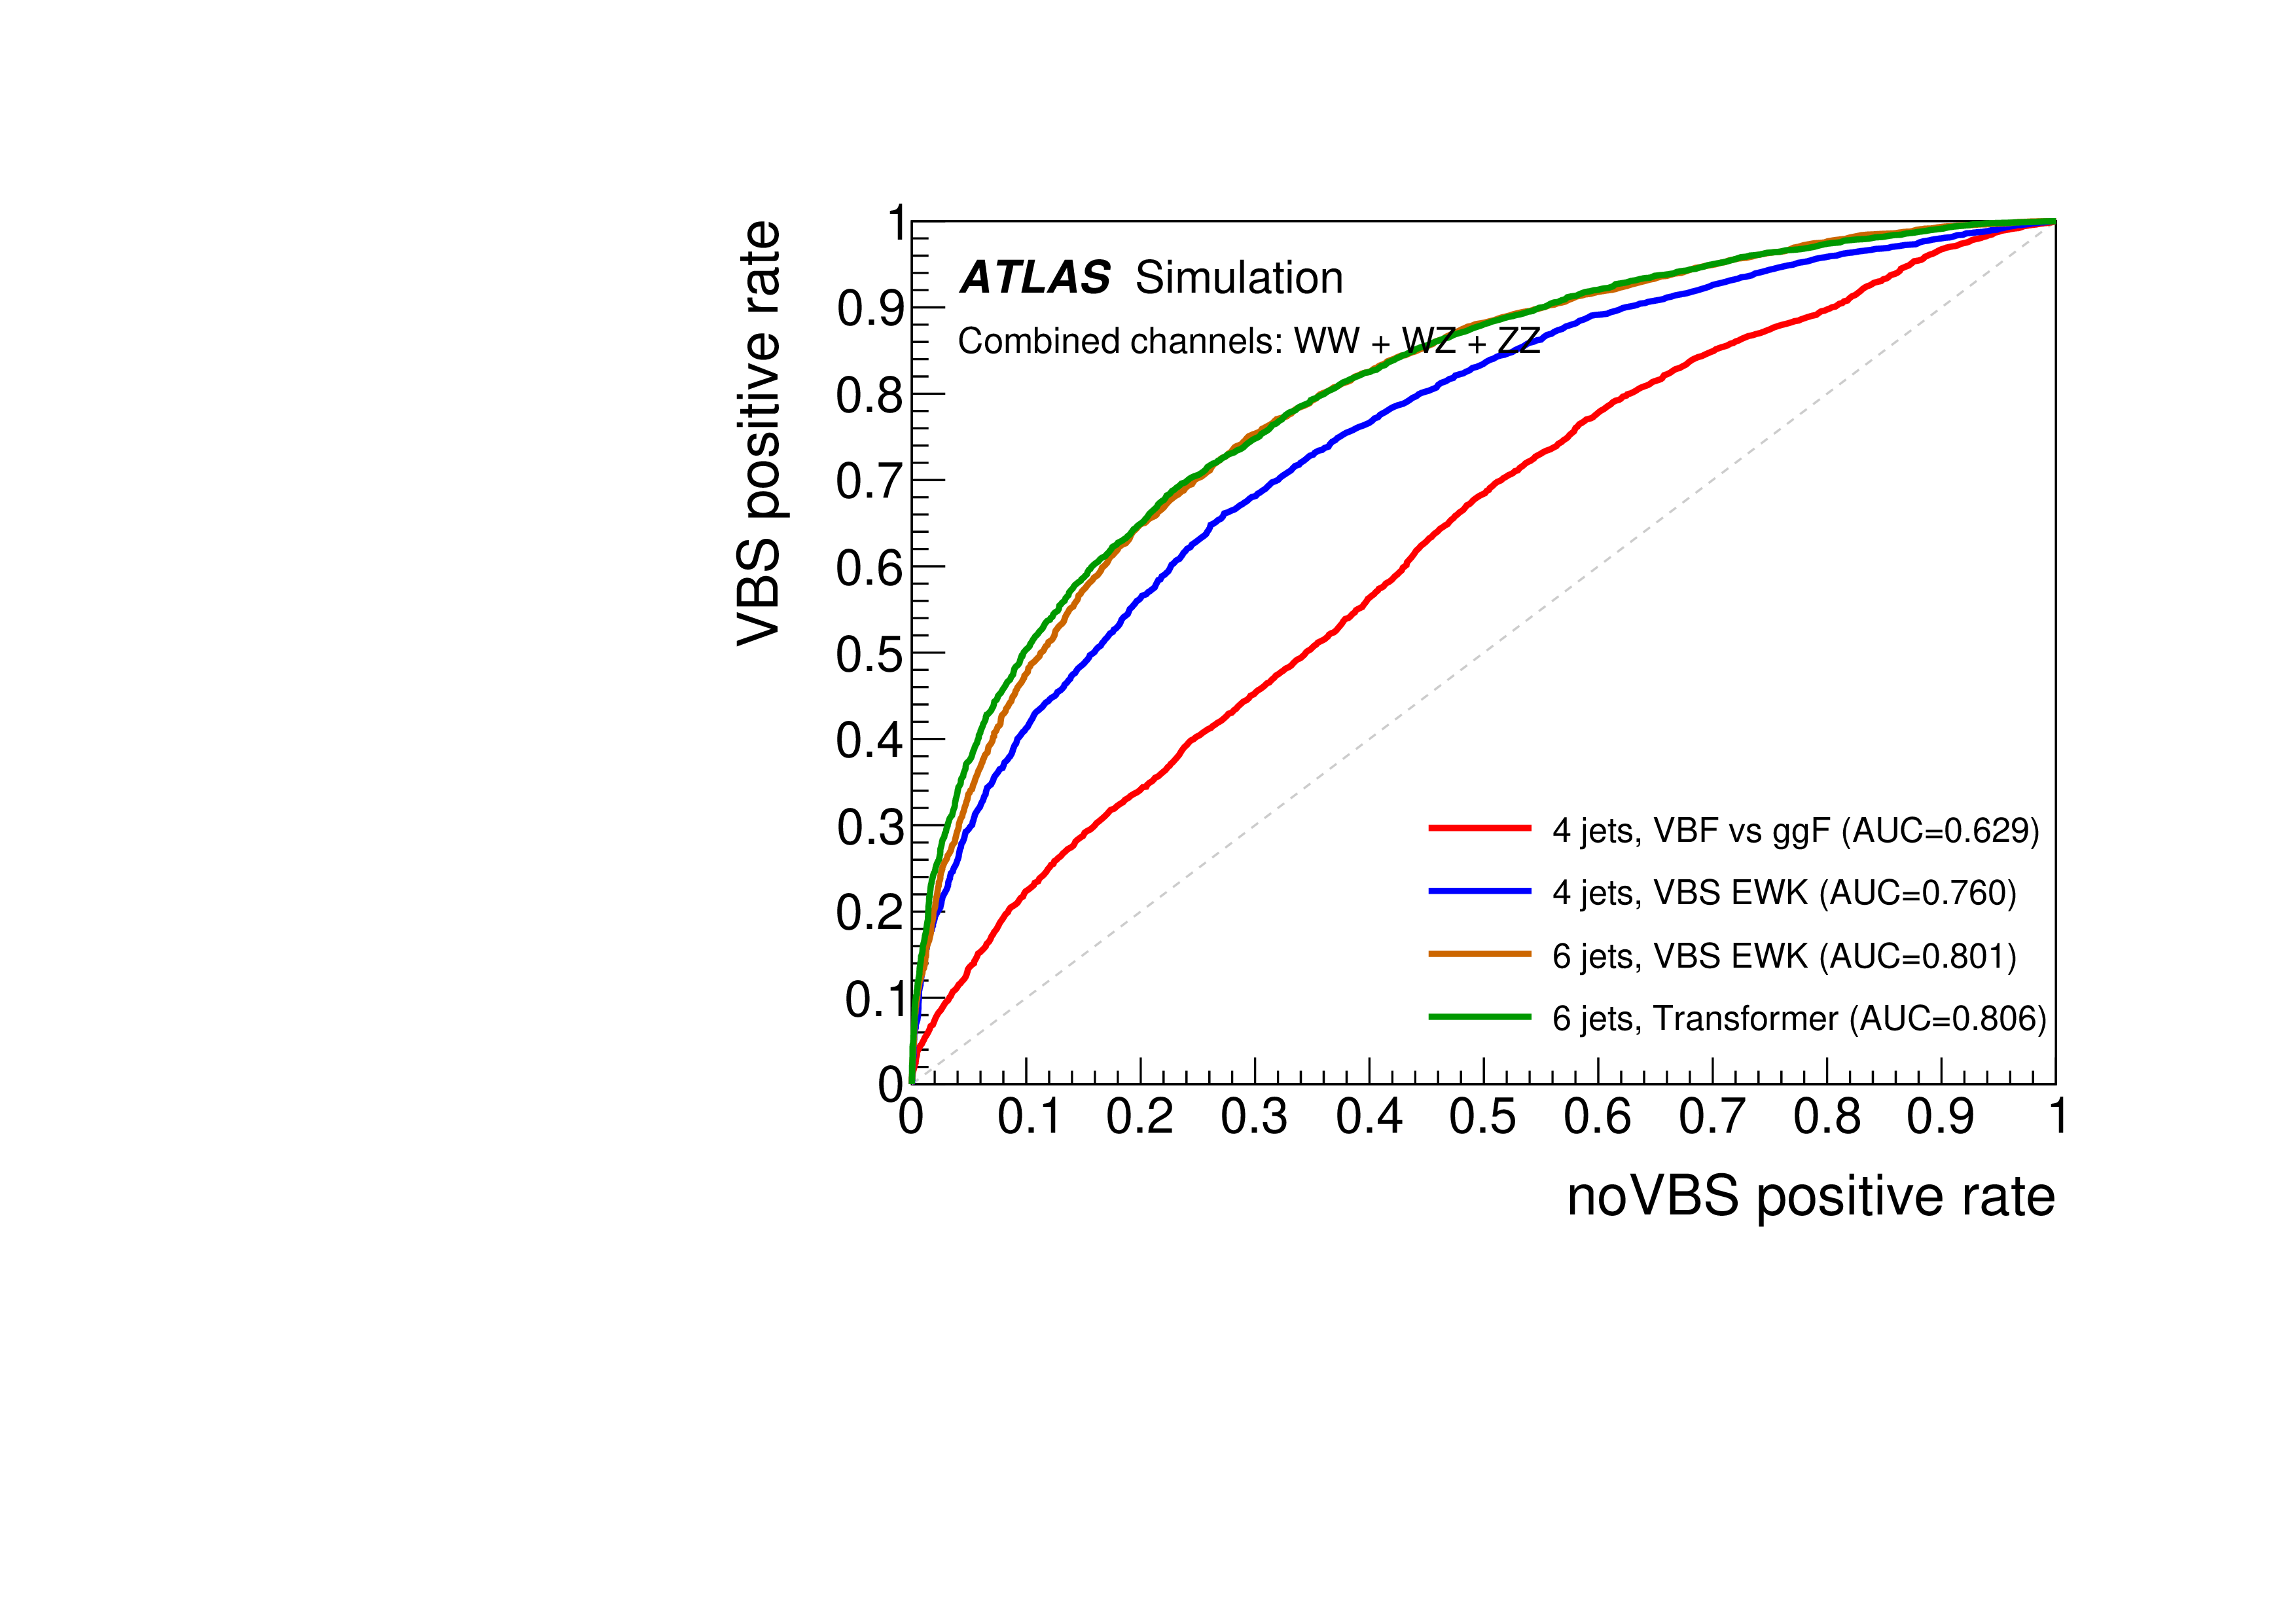
\includegraphics[width=0.7\textwidth]{figures/vbfrnn_roc_transformer.png}
\caption{ROC curves on the combined $WW+WZ+ZZ$ EWK validation sample, repeating the three RNN versions of Figure~\ref{fig:vbfrnn_roc} with the transformer added: version~1 ($\mathrm{AUC}=0.629$), version~2 ($\mathrm{AUC}=0.760$), version~3 ($\mathrm{AUC}=0.801$) and the six-jet transformer ($\mathrm{AUC}=0.806$). The transformer curve lies on top of the version~3 curve, confirming that the marginal AUC gain is not significant at high VBS efficiency.}
\label{fig:vbfrnn_roc_transformer}
\end{figure}

\section{Response to the aQGC operator families}
\label{sec:vbfrnn_aqgc}

The tagger is trained on inclusive electroweak $VVjj$ production rather than on any specific anomalous coupling, so it is essential to verify that it identifies the VBS topology consistently across the scalar, mixed and tensor aQGC operator families introduced in Chapter~\ref{chap:sm}, since these families excite different gauge-boson polarisation modes and could in principle populate the score differently.

Figure~\ref{fig:vbfrnn_aqgc_v1} shows the response of version~1 to representative scalar ($S_{0,1}$), tensor ($T_{0,1}$) and mixed ($M_{0,1}$) operators. While the scalar operators are pushed to high scores, the tensor and mixed operators peak at low scores: the resonance-trained tagger fails to recognise the VBS topology of the transverse-polarisation-dominated operators, mirroring its poor inclusive AUC. Figures~\ref{fig:vbfrnn_aqgc_v2} and~\ref{fig:vbfrnn_aqgc_v3} show the same operators for version~2 and version~3 respectively. Version~2 already yields broad responses peaking at intermediate-to-high scores for all three families, with the multiplicity artefact discussed in Section~\ref{sec:vbfrnn_multiplicity} still visible. Version~3 produces a clean response strongly peaked near $s\approx1$ for every operator family, demonstrating that the six-jet tagger identifies the VBS topology uniformly regardless of the underlying operator, without being biased towards any particular polarisation structure. This operator-independent response is what justifies using a single tagger, trained on inclusive EWK production, as a pre-selection requirement and as an input feature to the aQGC discriminant of Chapter~\ref{chap:analysismethods}.

\begin{figure}[h]
\centering
\begin{subfigure}[b]{0.32\textwidth}
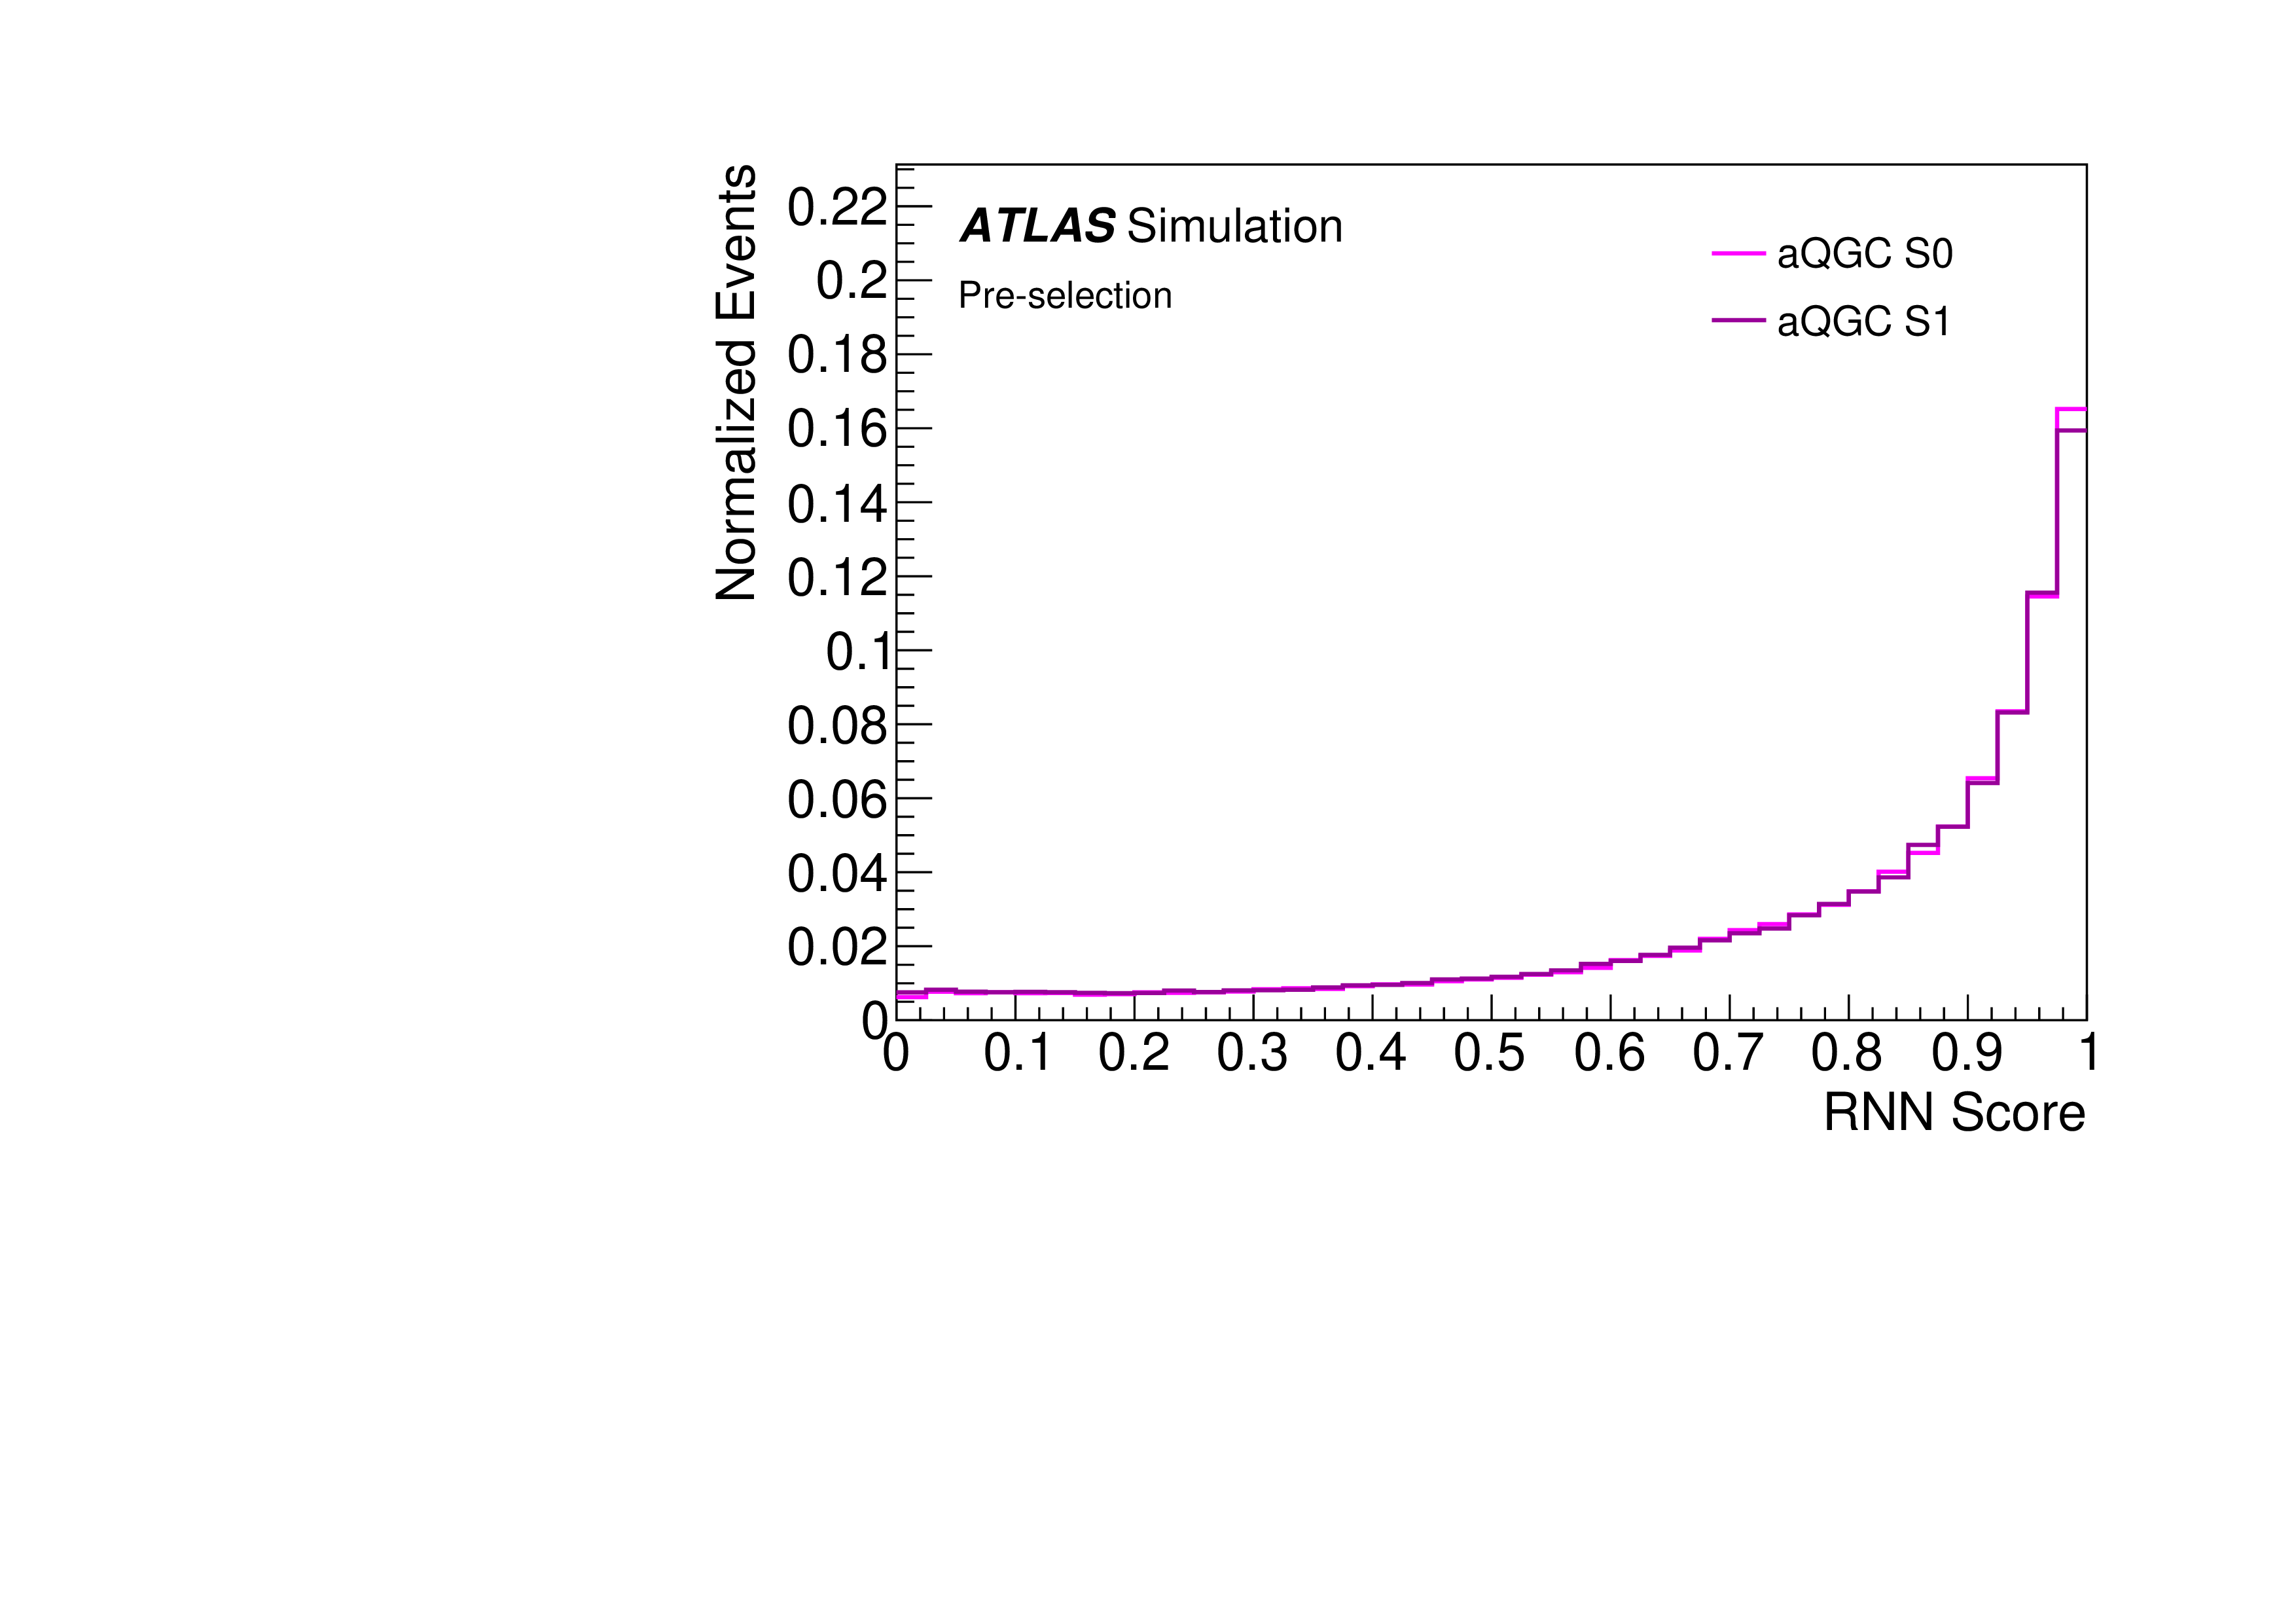
\includegraphics[width=\textwidth]{figures/vbfrnn_aqgc_v1_S.png}
\caption{Scalar}
\end{subfigure}
\begin{subfigure}[b]{0.32\textwidth}
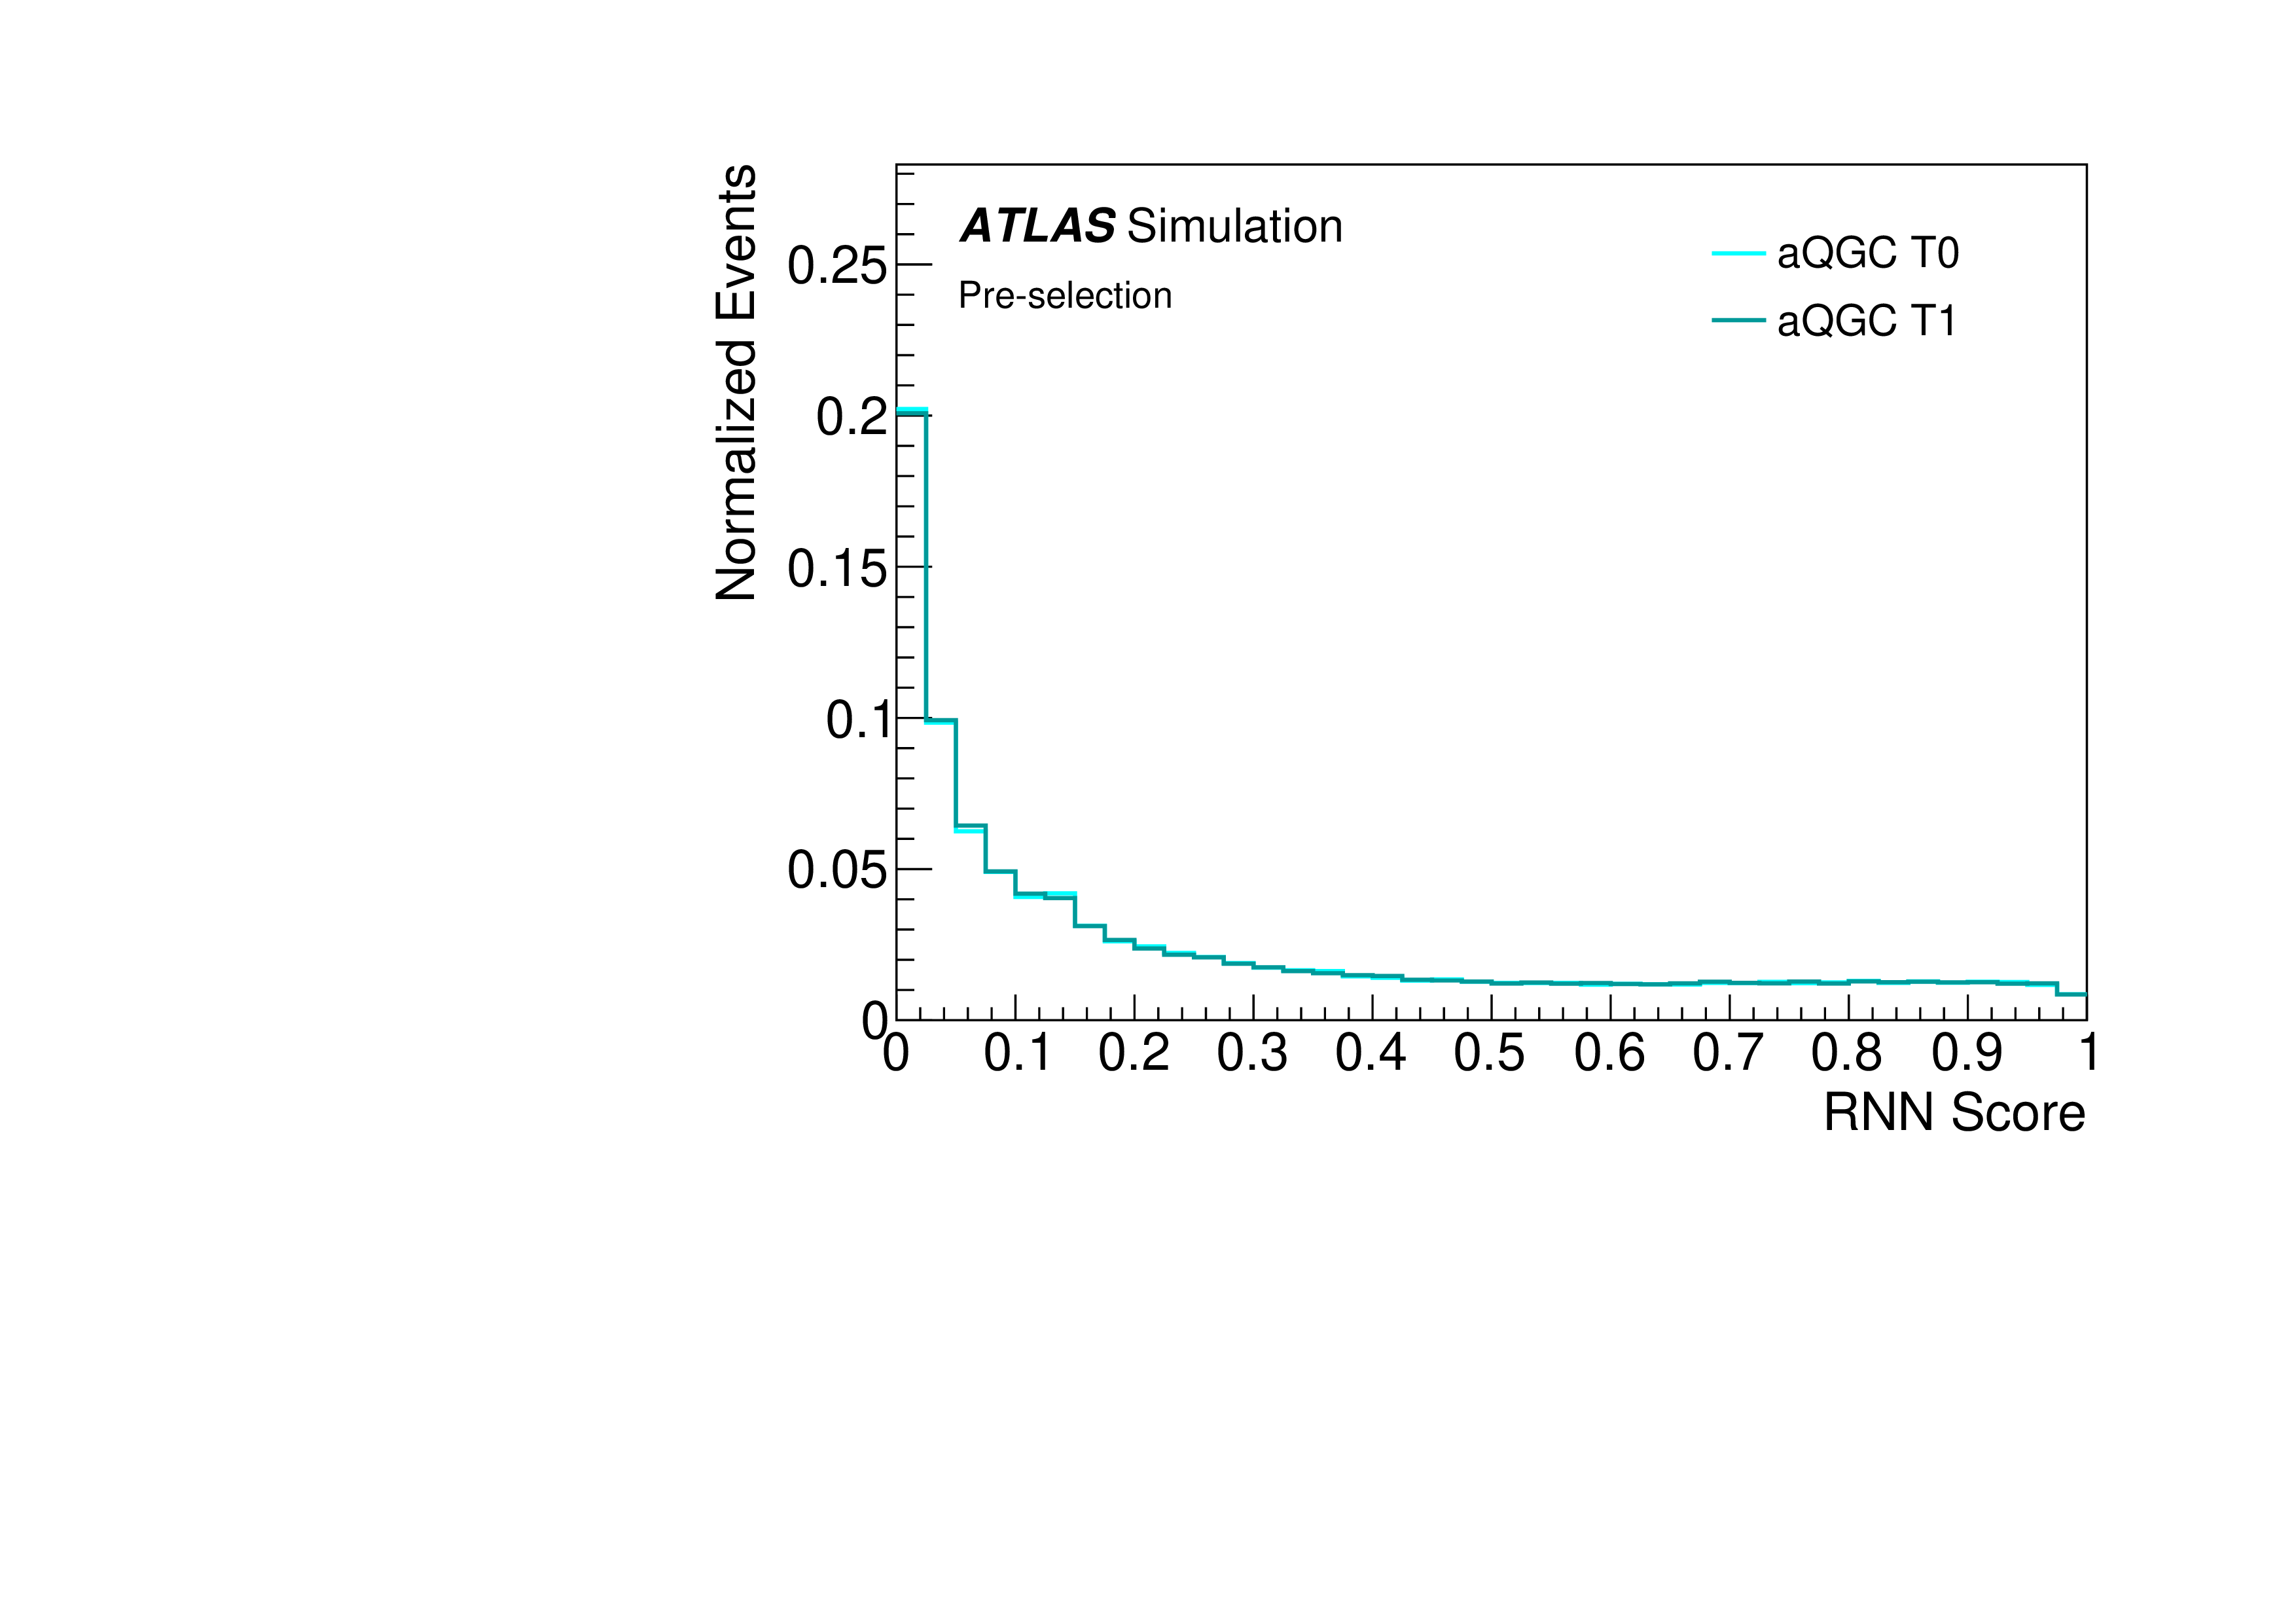
\includegraphics[width=\textwidth]{figures/vbfrnn_aqgc_v1_T.png}
\caption{Tensor}
\end{subfigure}
\begin{subfigure}[b]{0.32\textwidth}
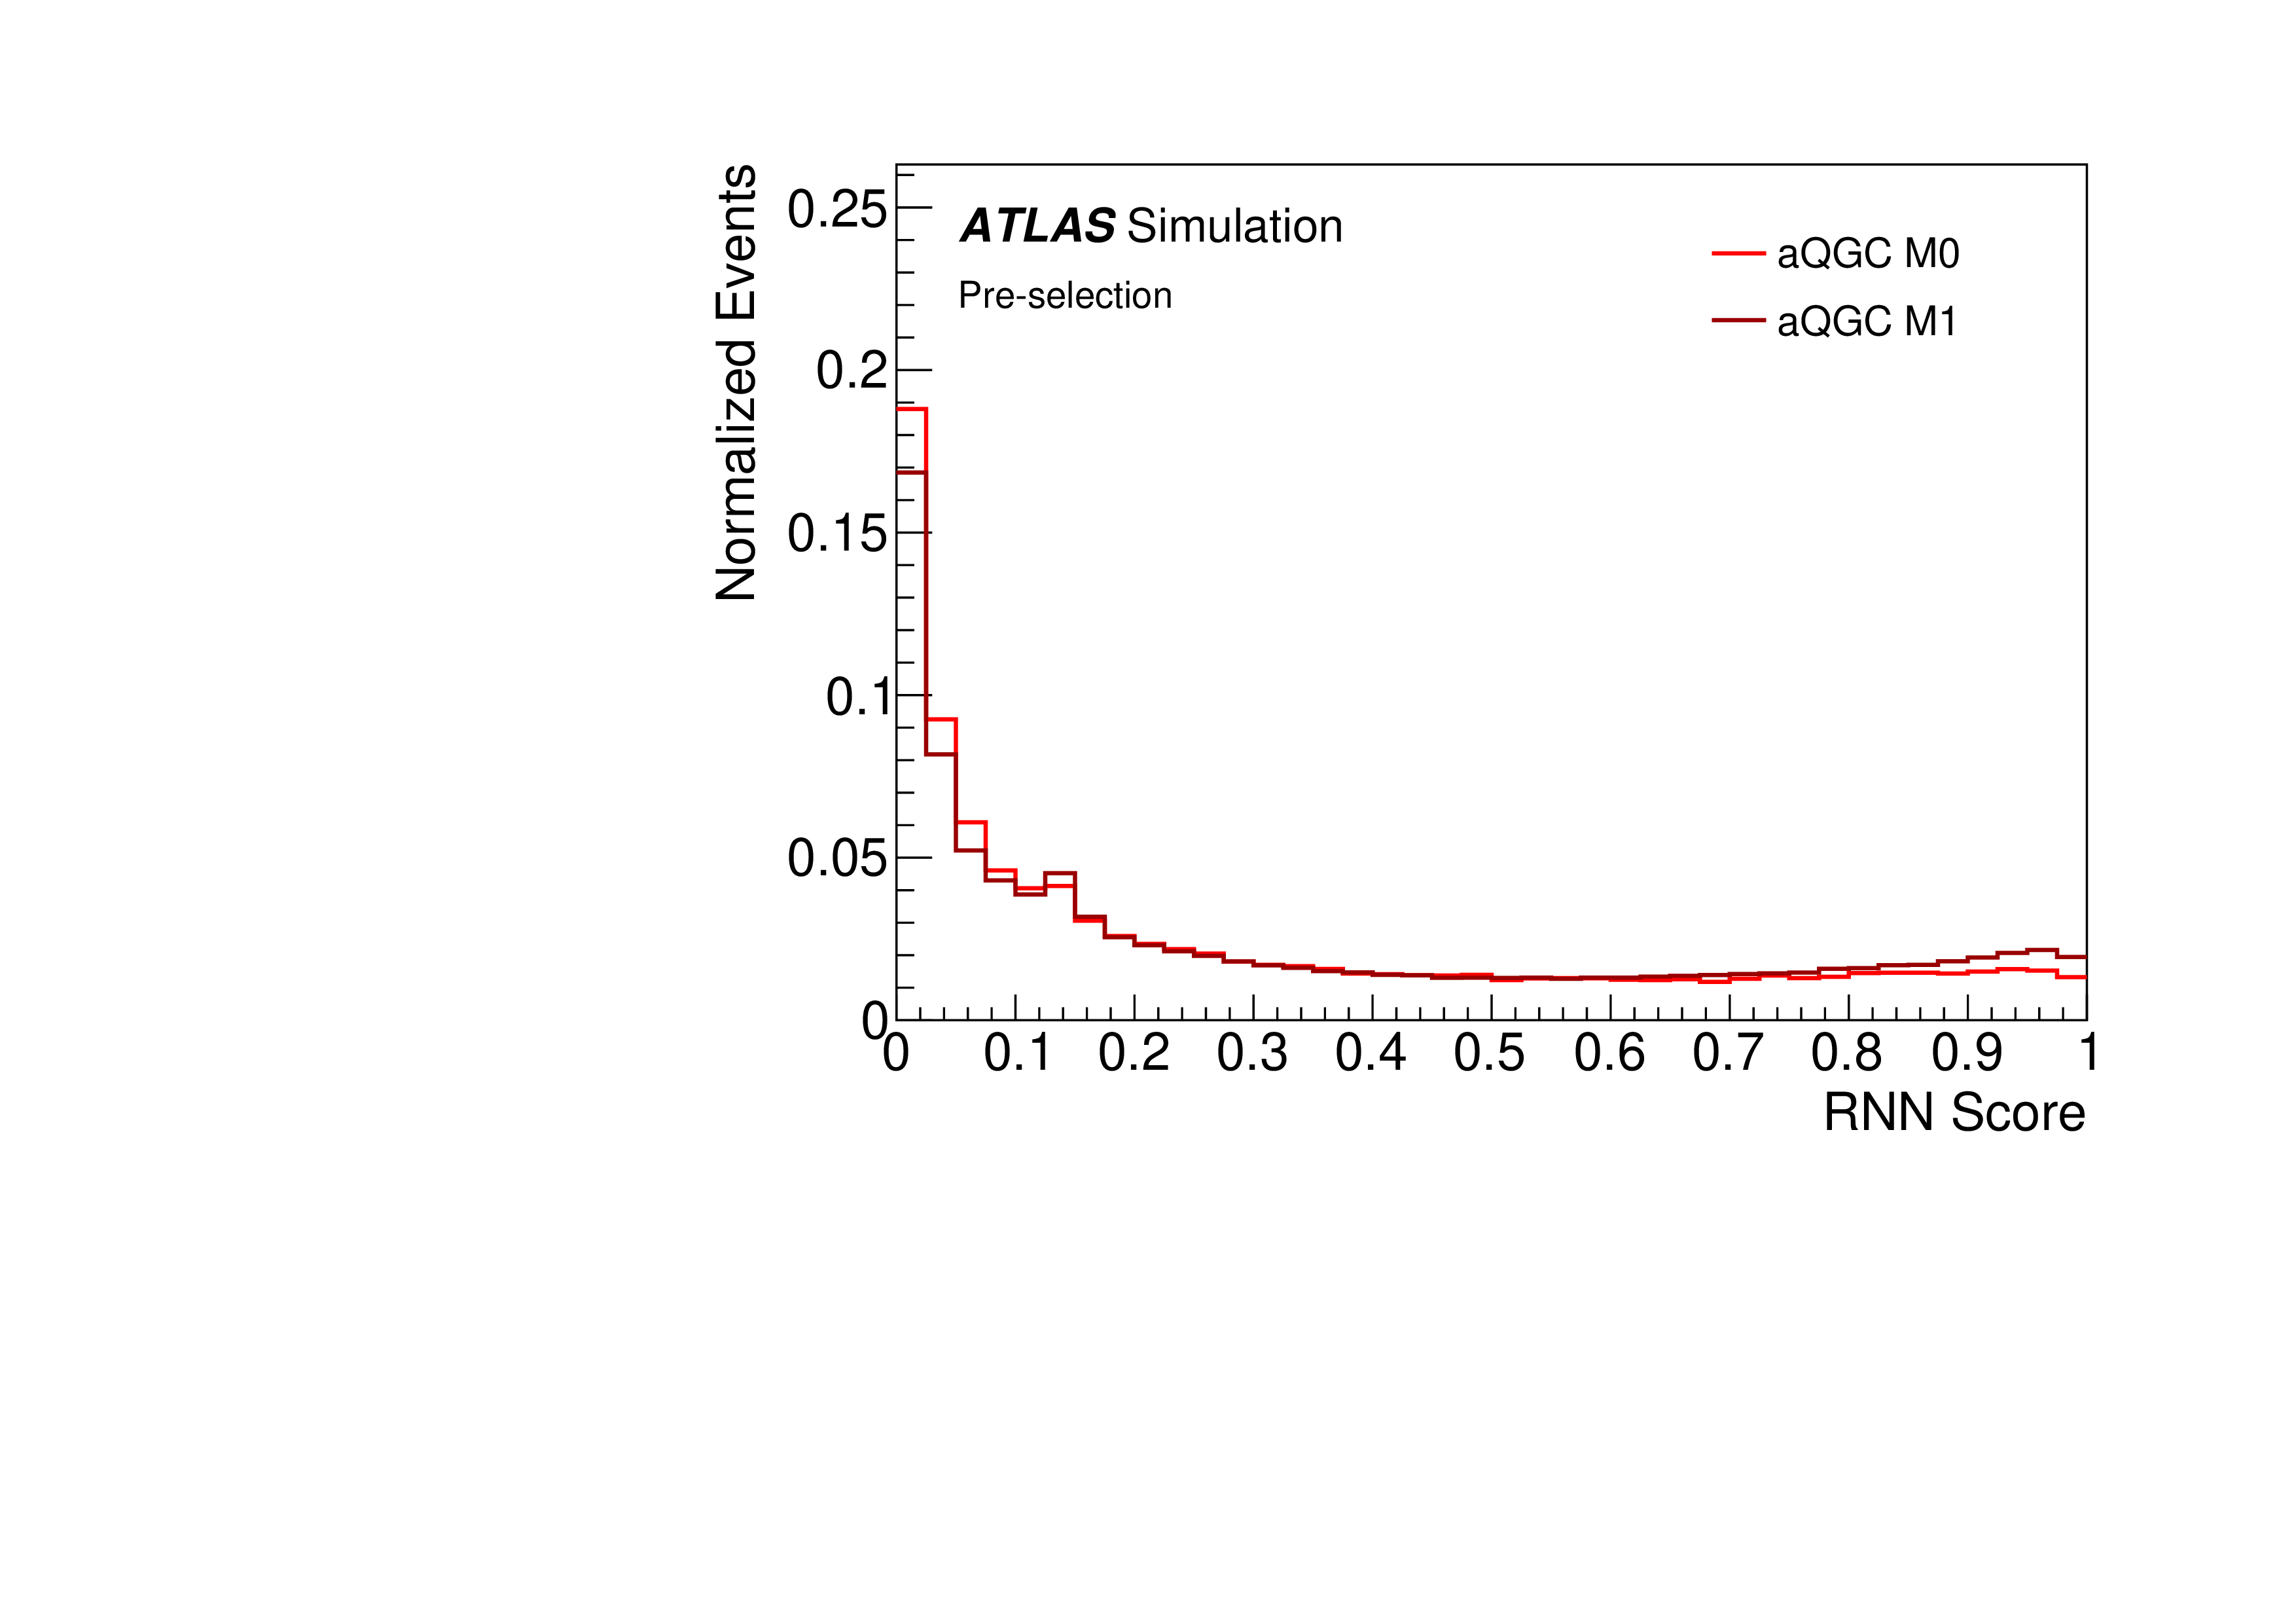
\includegraphics[width=\textwidth]{figures/vbfrnn_aqgc_v1_M.png}
\caption{Mixed}
\end{subfigure}
\caption{Normalised version~1 (4 jets, VBF vs.\ ggF) RNN score for representative scalar ($S_0$, $S_1$), tensor ($T_0$, $T_1$) and mixed ($M_0$, $M_1$) aQGC operators. The resonance-trained tagger separates the scalar operators well but assigns low scores to the tensor and mixed operators.}
\label{fig:vbfrnn_aqgc_v1}
\end{figure}

\begin{figure}[h]
\centering
\begin{subfigure}[b]{0.32\textwidth}
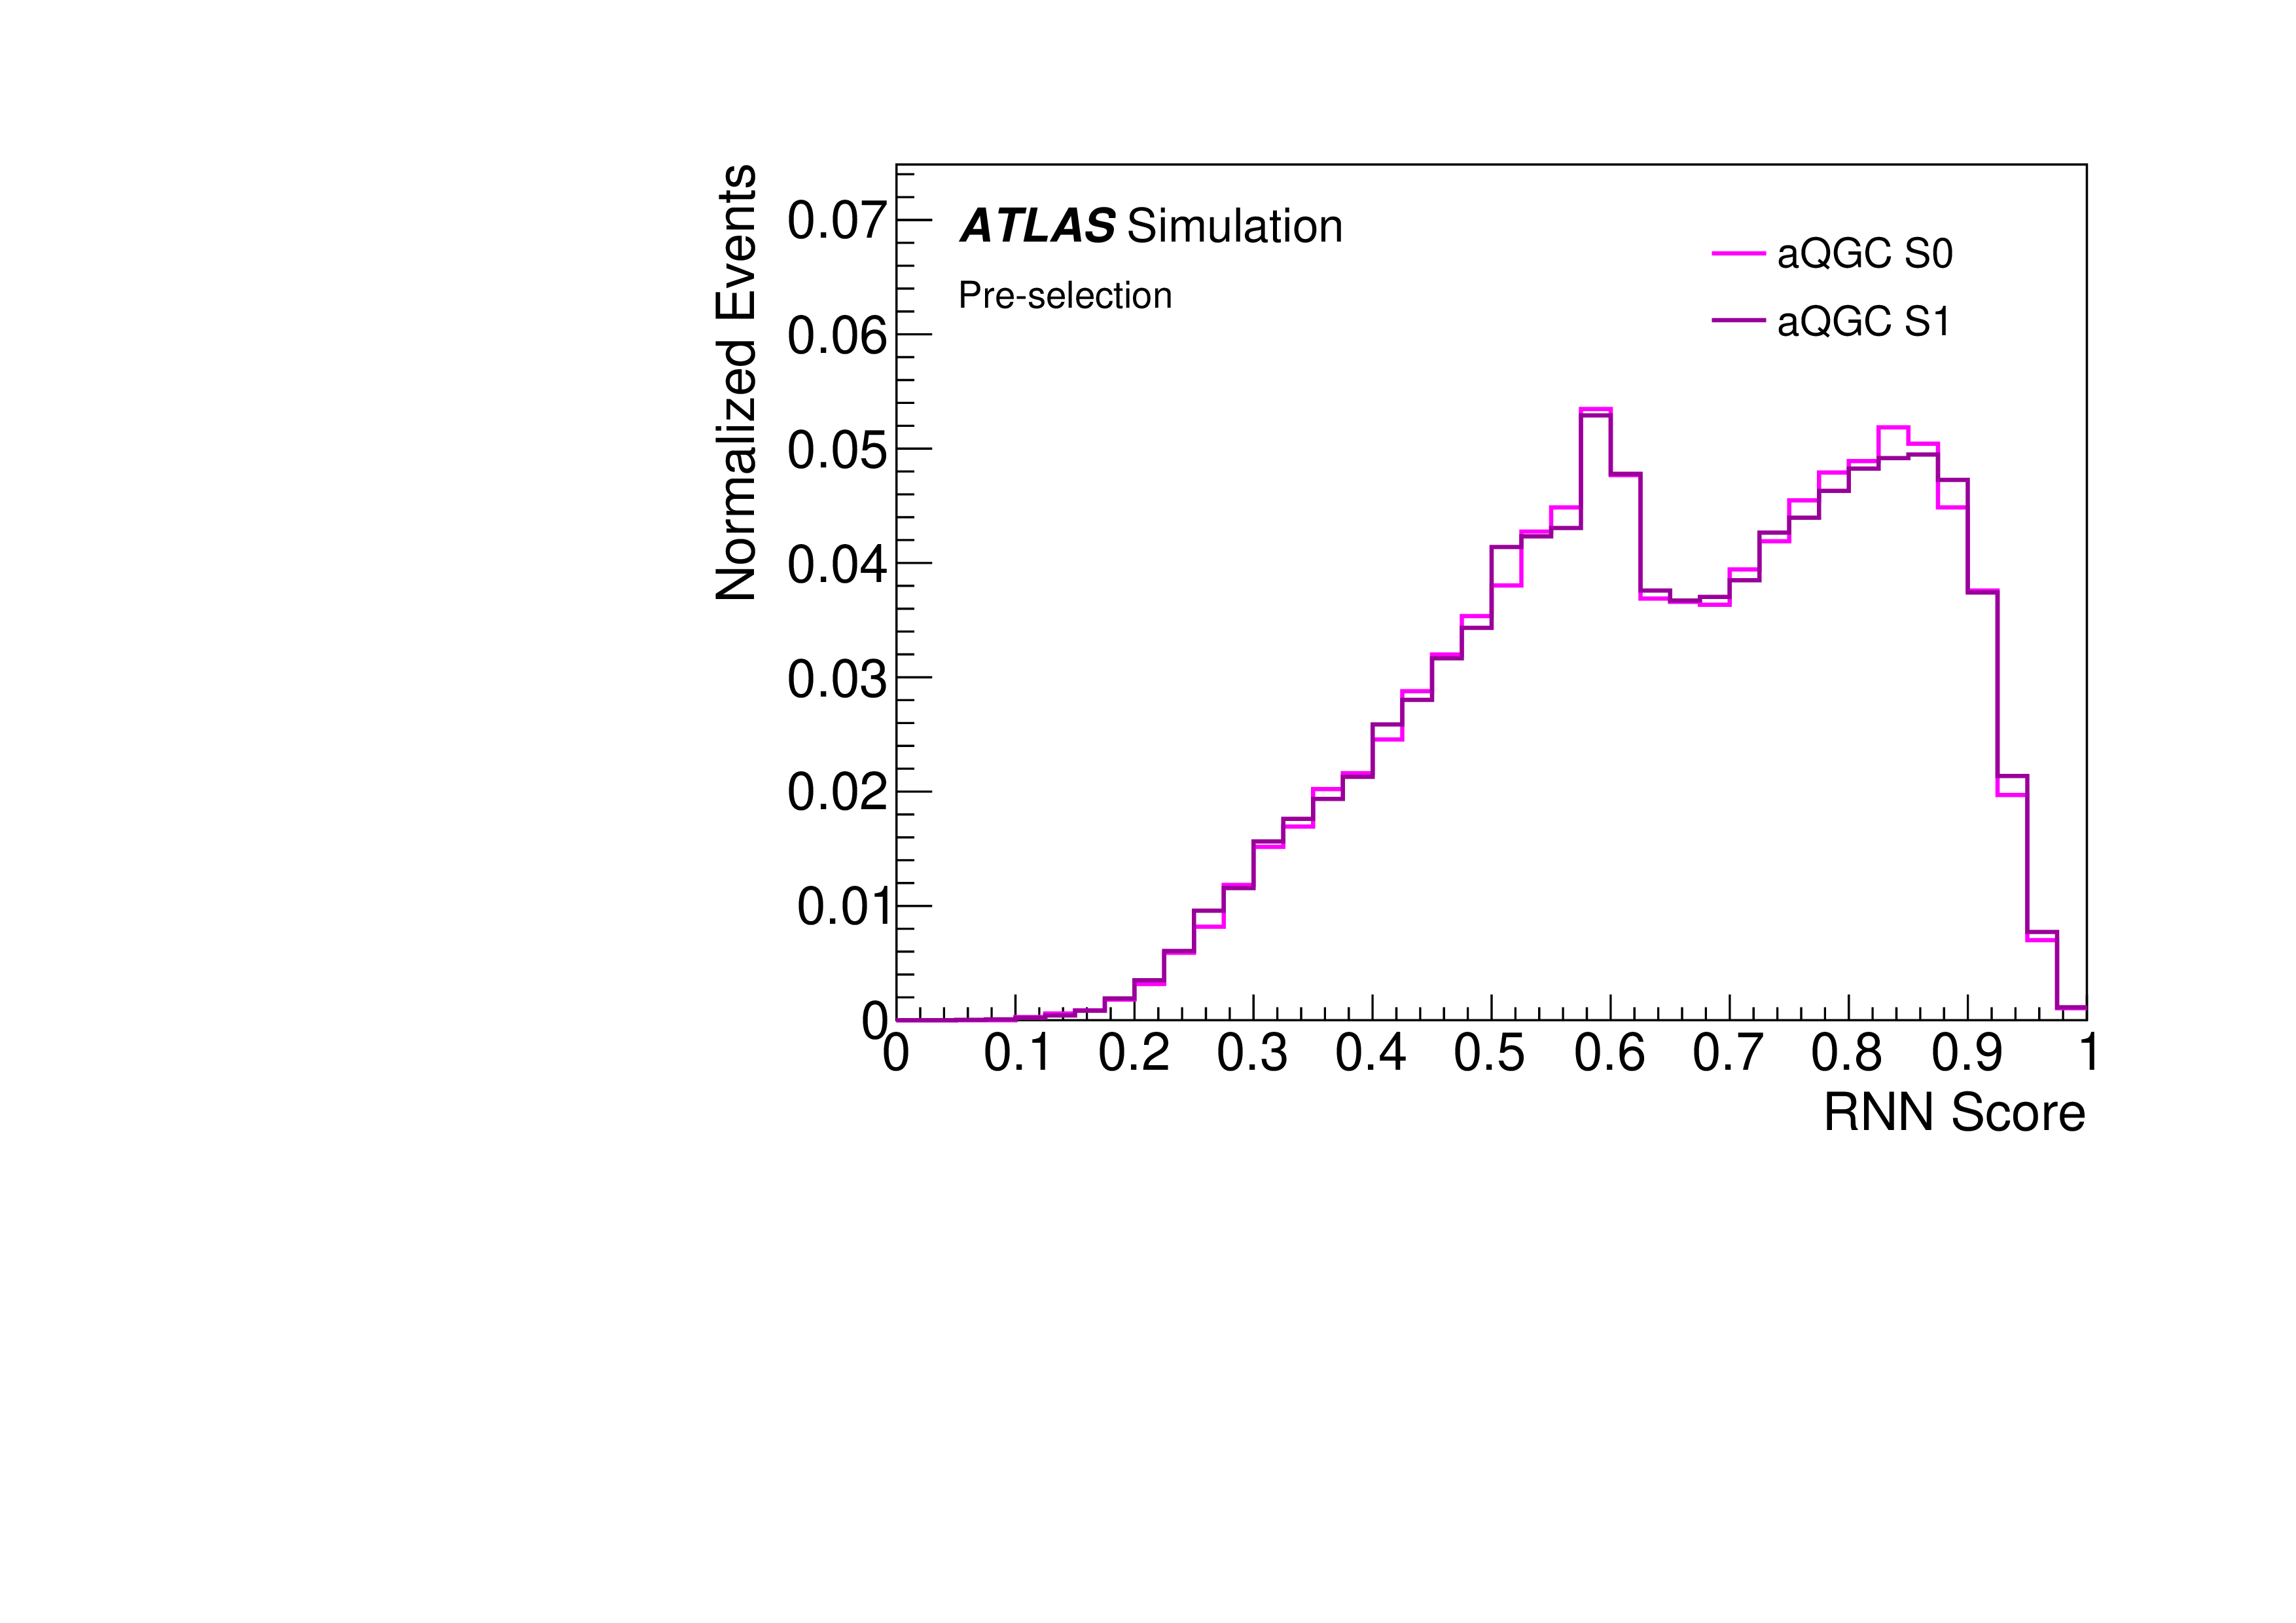
\includegraphics[width=\textwidth]{figures/vbfrnn_aqgc_v2_S.png}
\caption{Scalar}
\end{subfigure}
\begin{subfigure}[b]{0.32\textwidth}
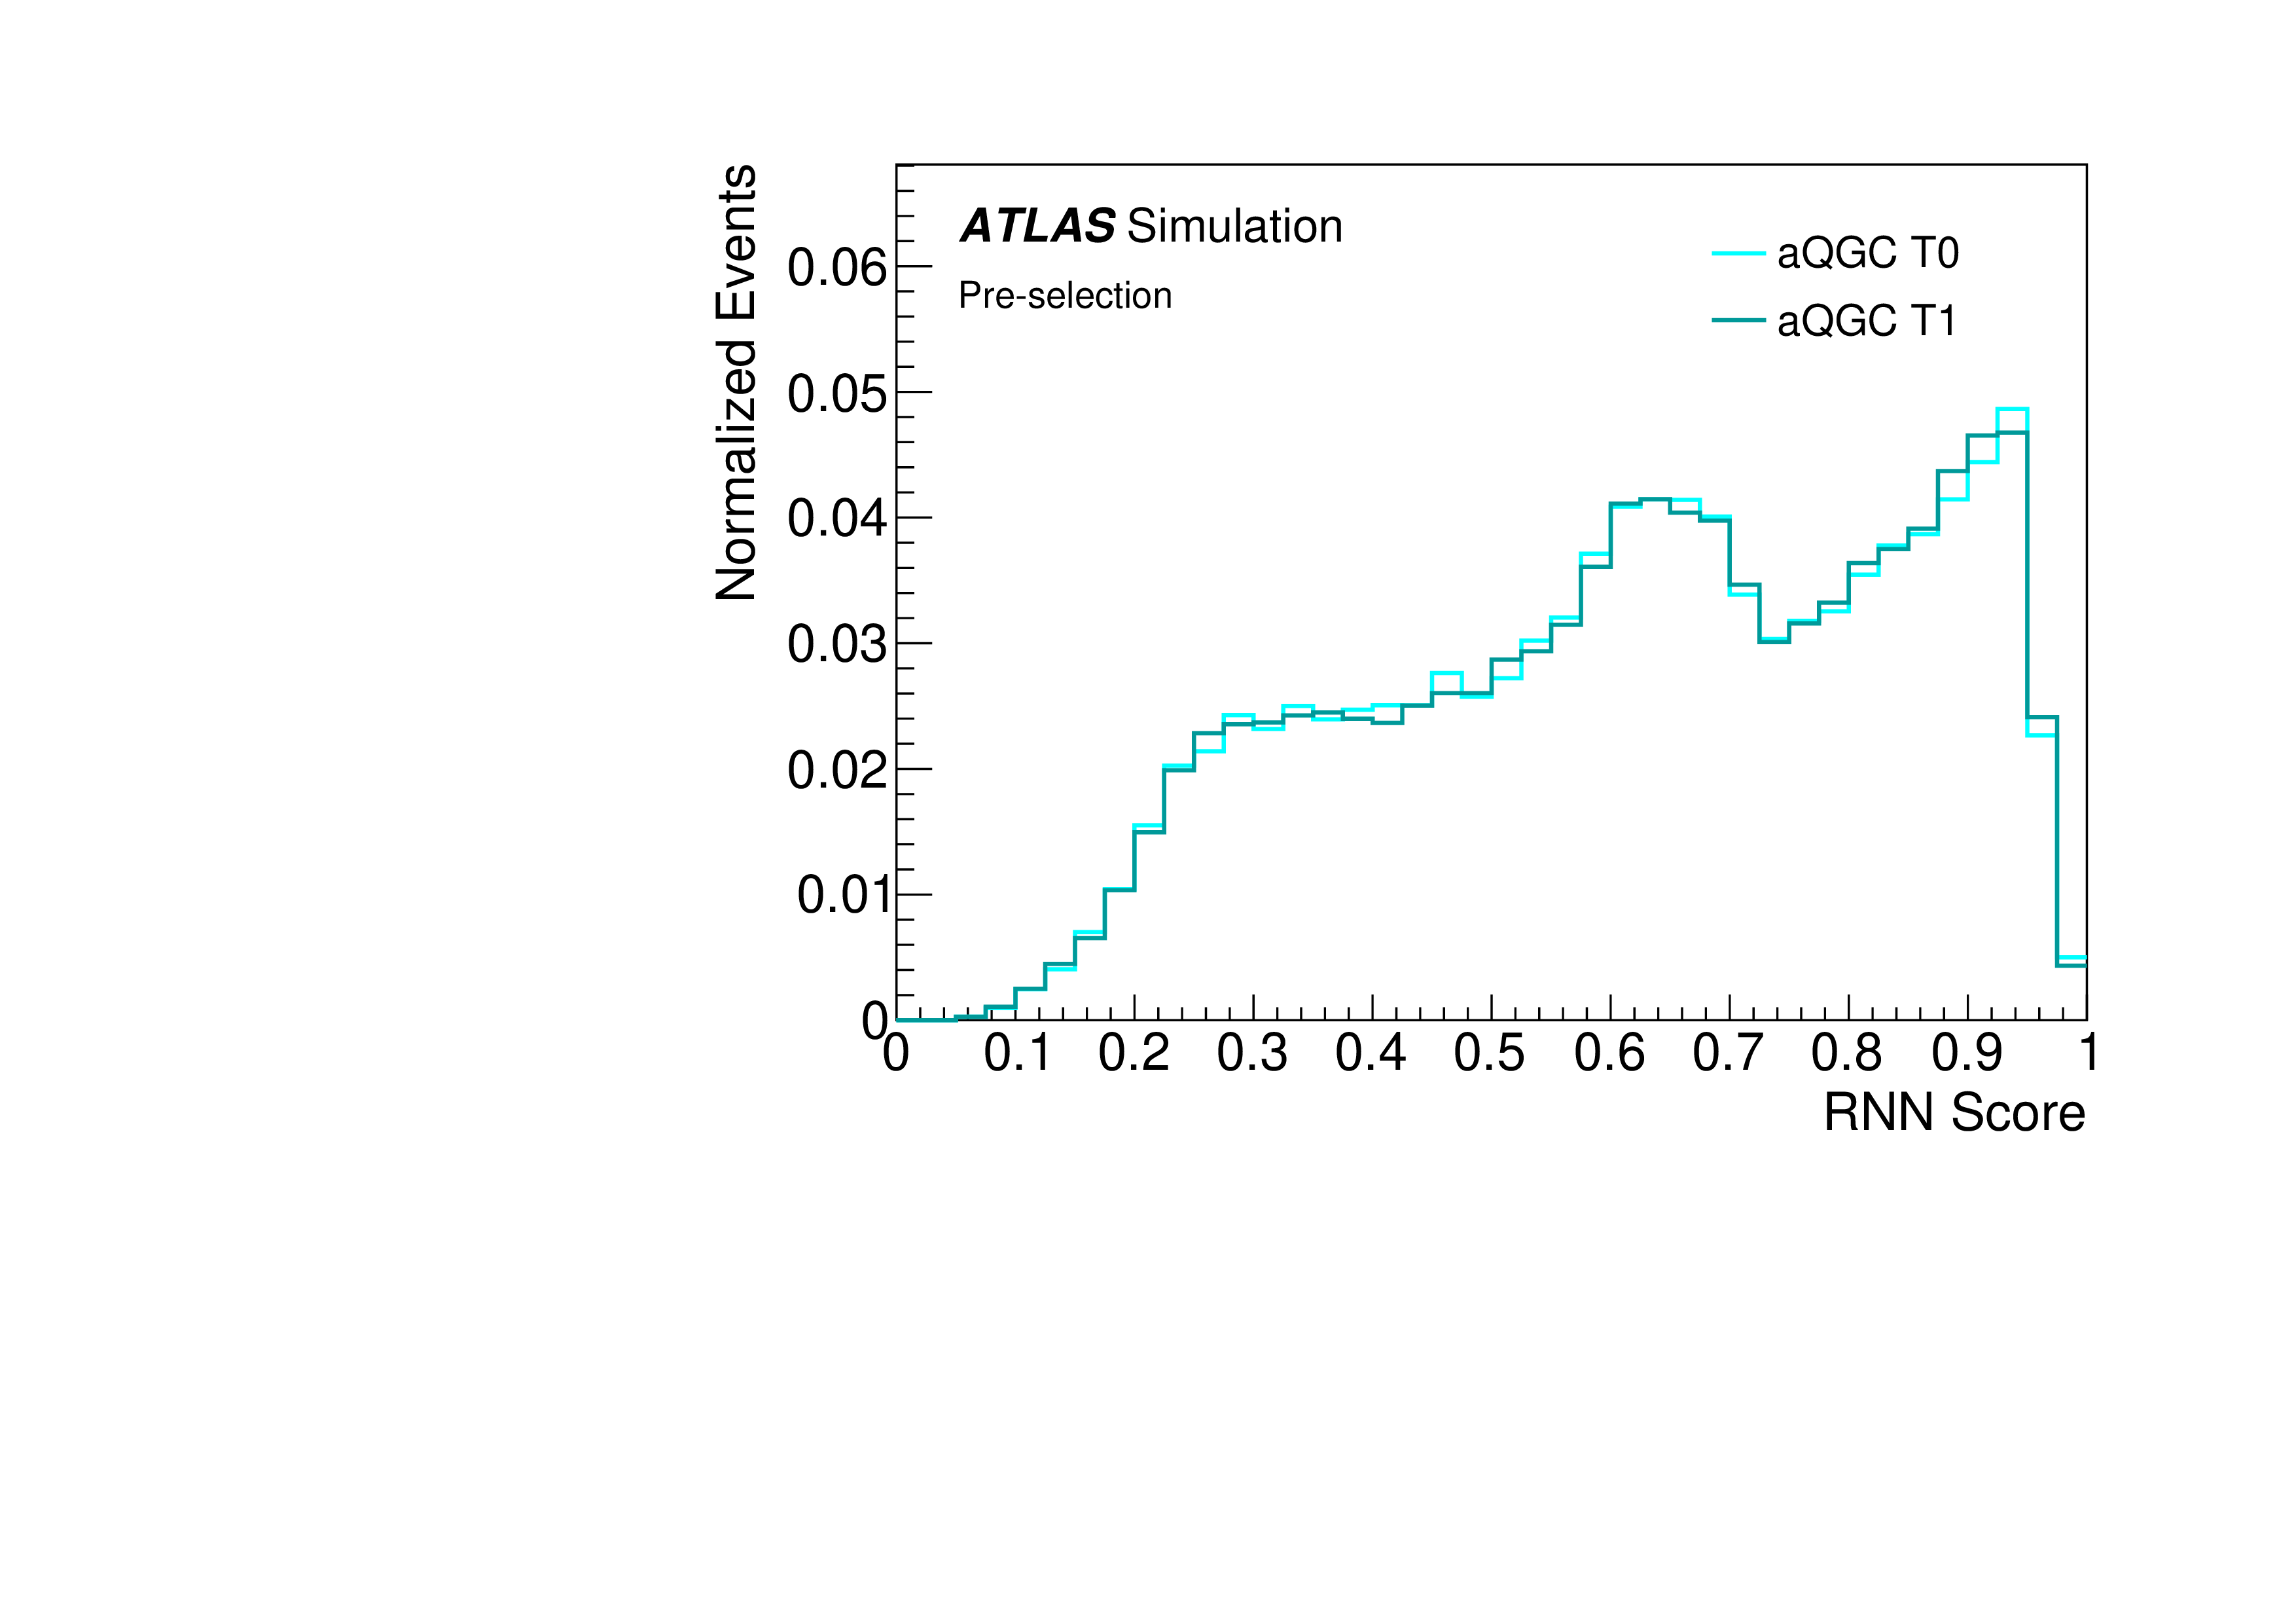
\includegraphics[width=\textwidth]{figures/vbfrnn_aqgc_v2_T.png}
\caption{Tensor}
\end{subfigure}
\begin{subfigure}[b]{0.32\textwidth}
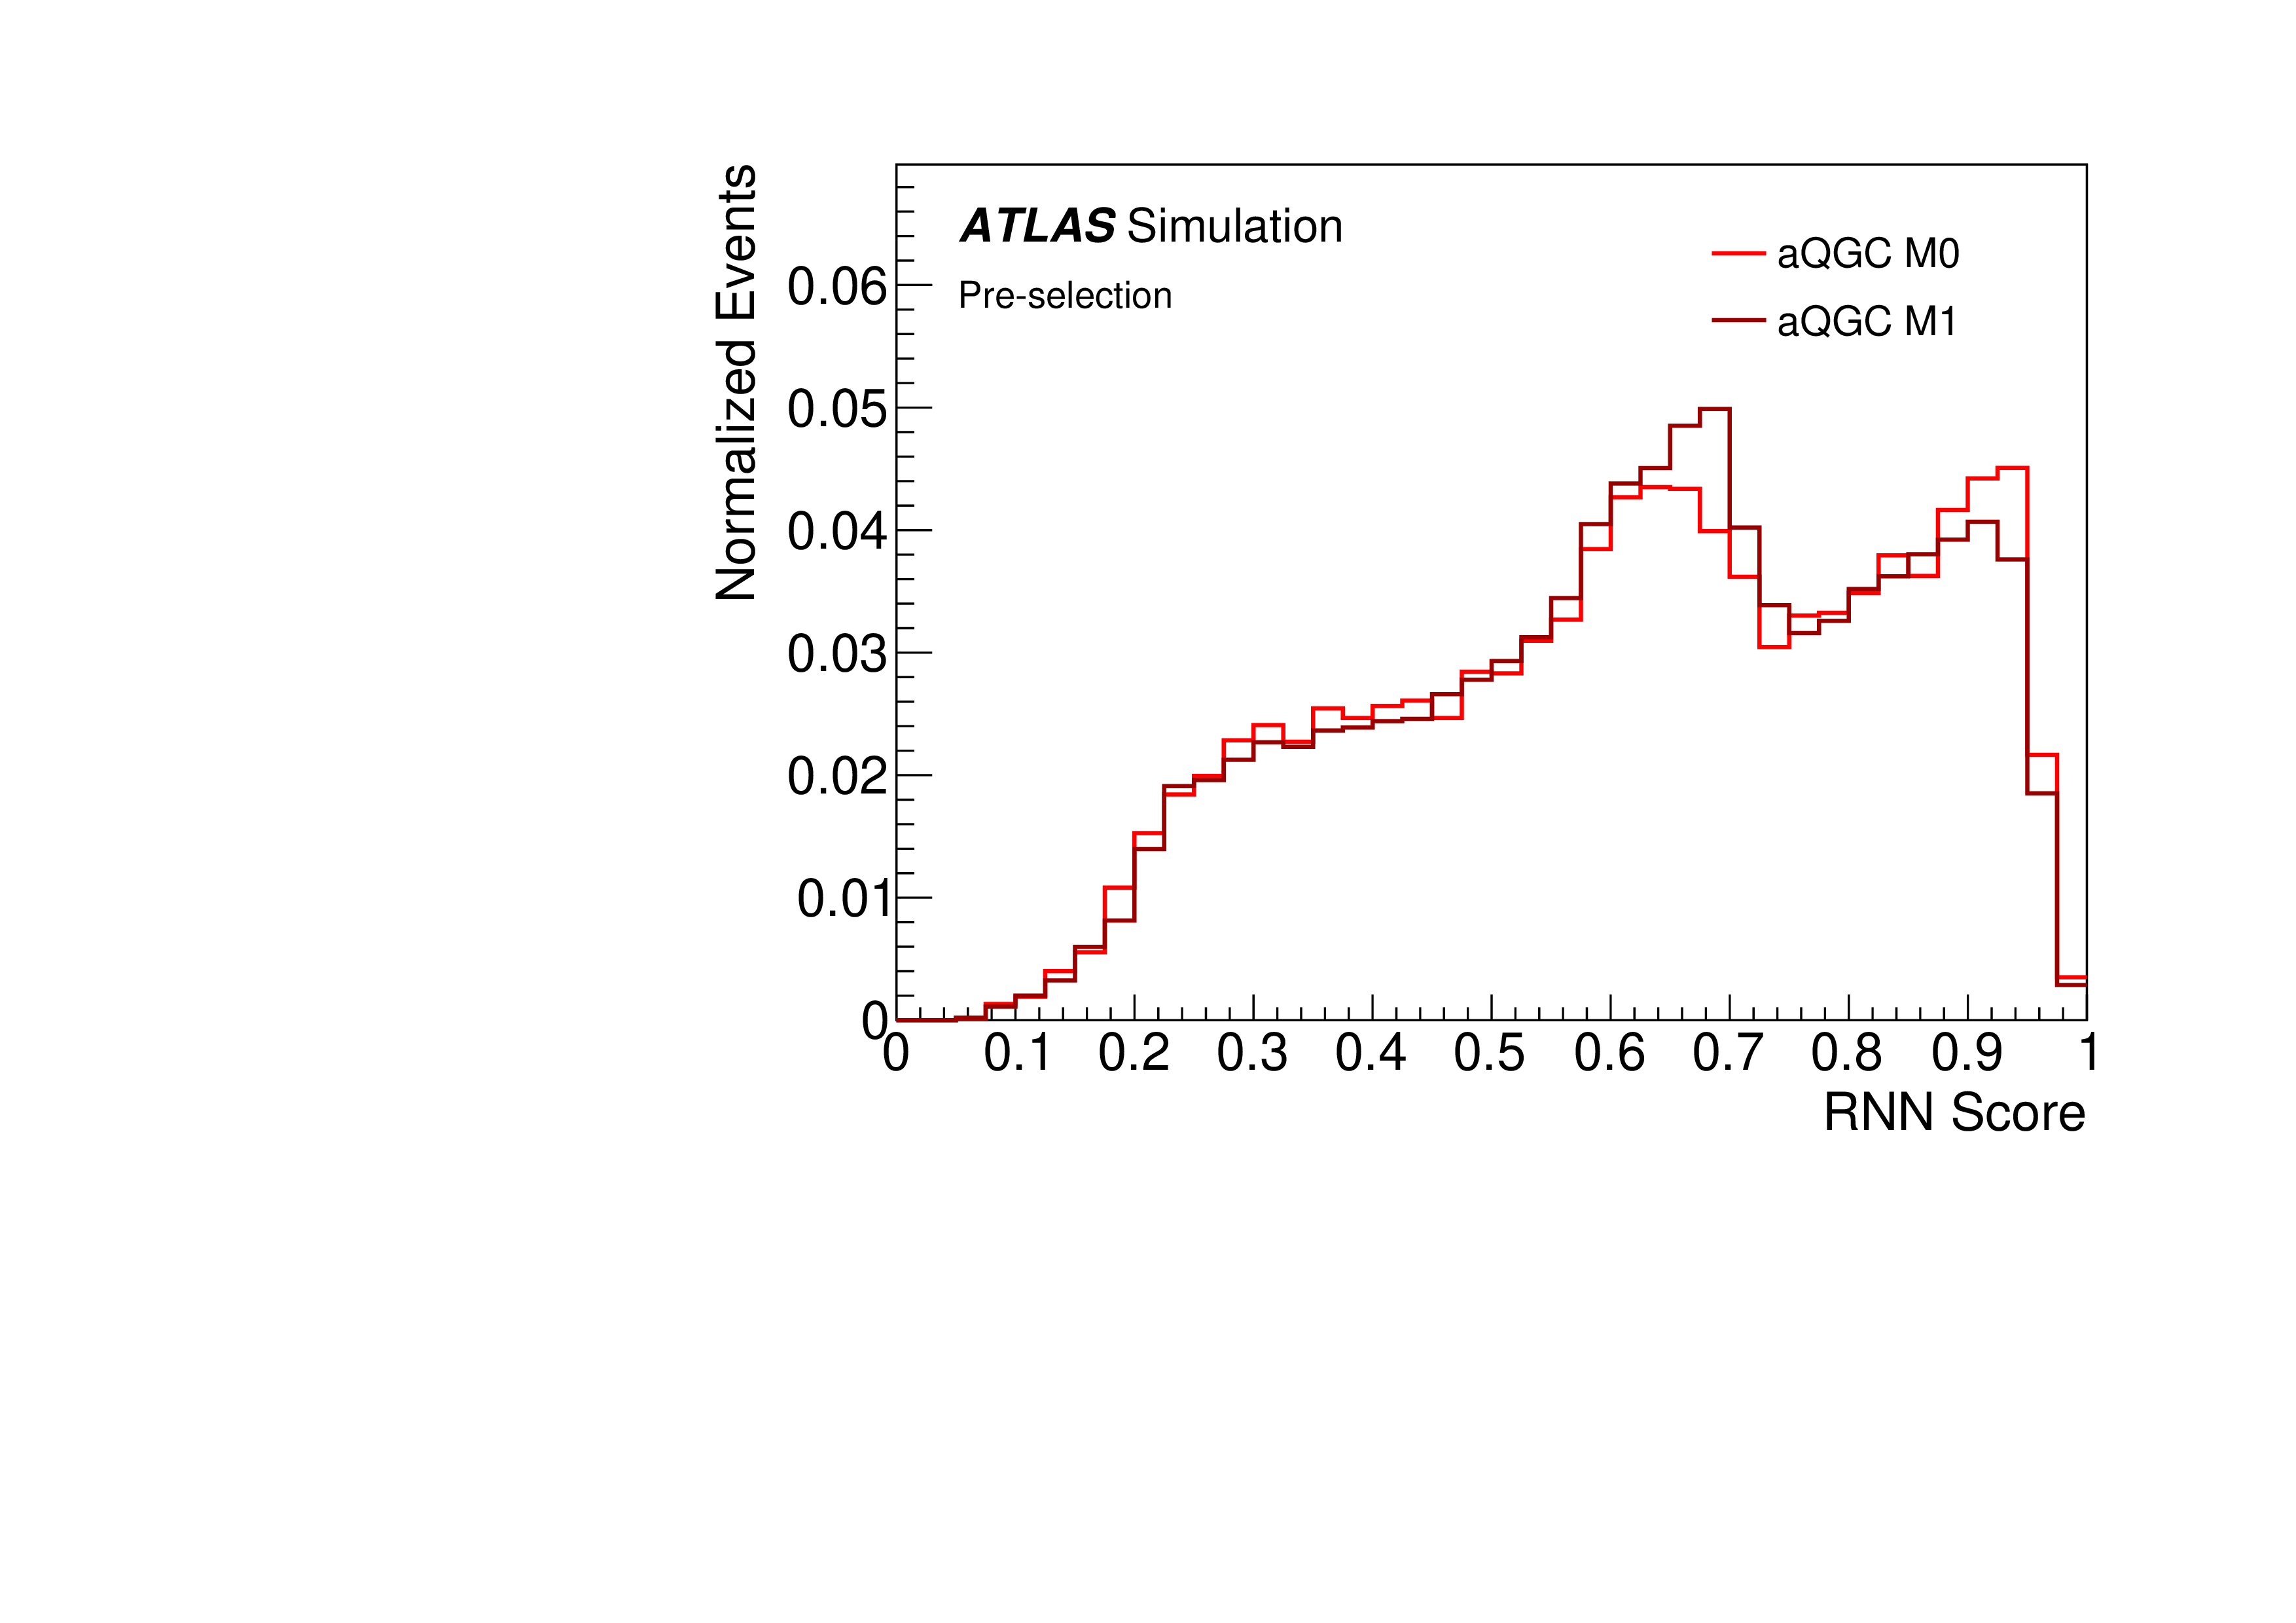
\includegraphics[width=\textwidth]{figures/vbfrnn_aqgc_v2_M.png}
\caption{Mixed}
\end{subfigure}
\caption{Normalised version~2 (4 jets, VBS vs.\ non-VBS EWK) RNN score for representative scalar, tensor and mixed aQGC operators. The response peaks at intermediate-to-high scores for all three families, with the input-multiplicity artefact of Section~\ref{sec:vbfrnn_multiplicity} still visible.}
\label{fig:vbfrnn_aqgc_v2}
\end{figure}

\begin{figure}[h]
\centering
\begin{subfigure}[b]{0.32\textwidth}
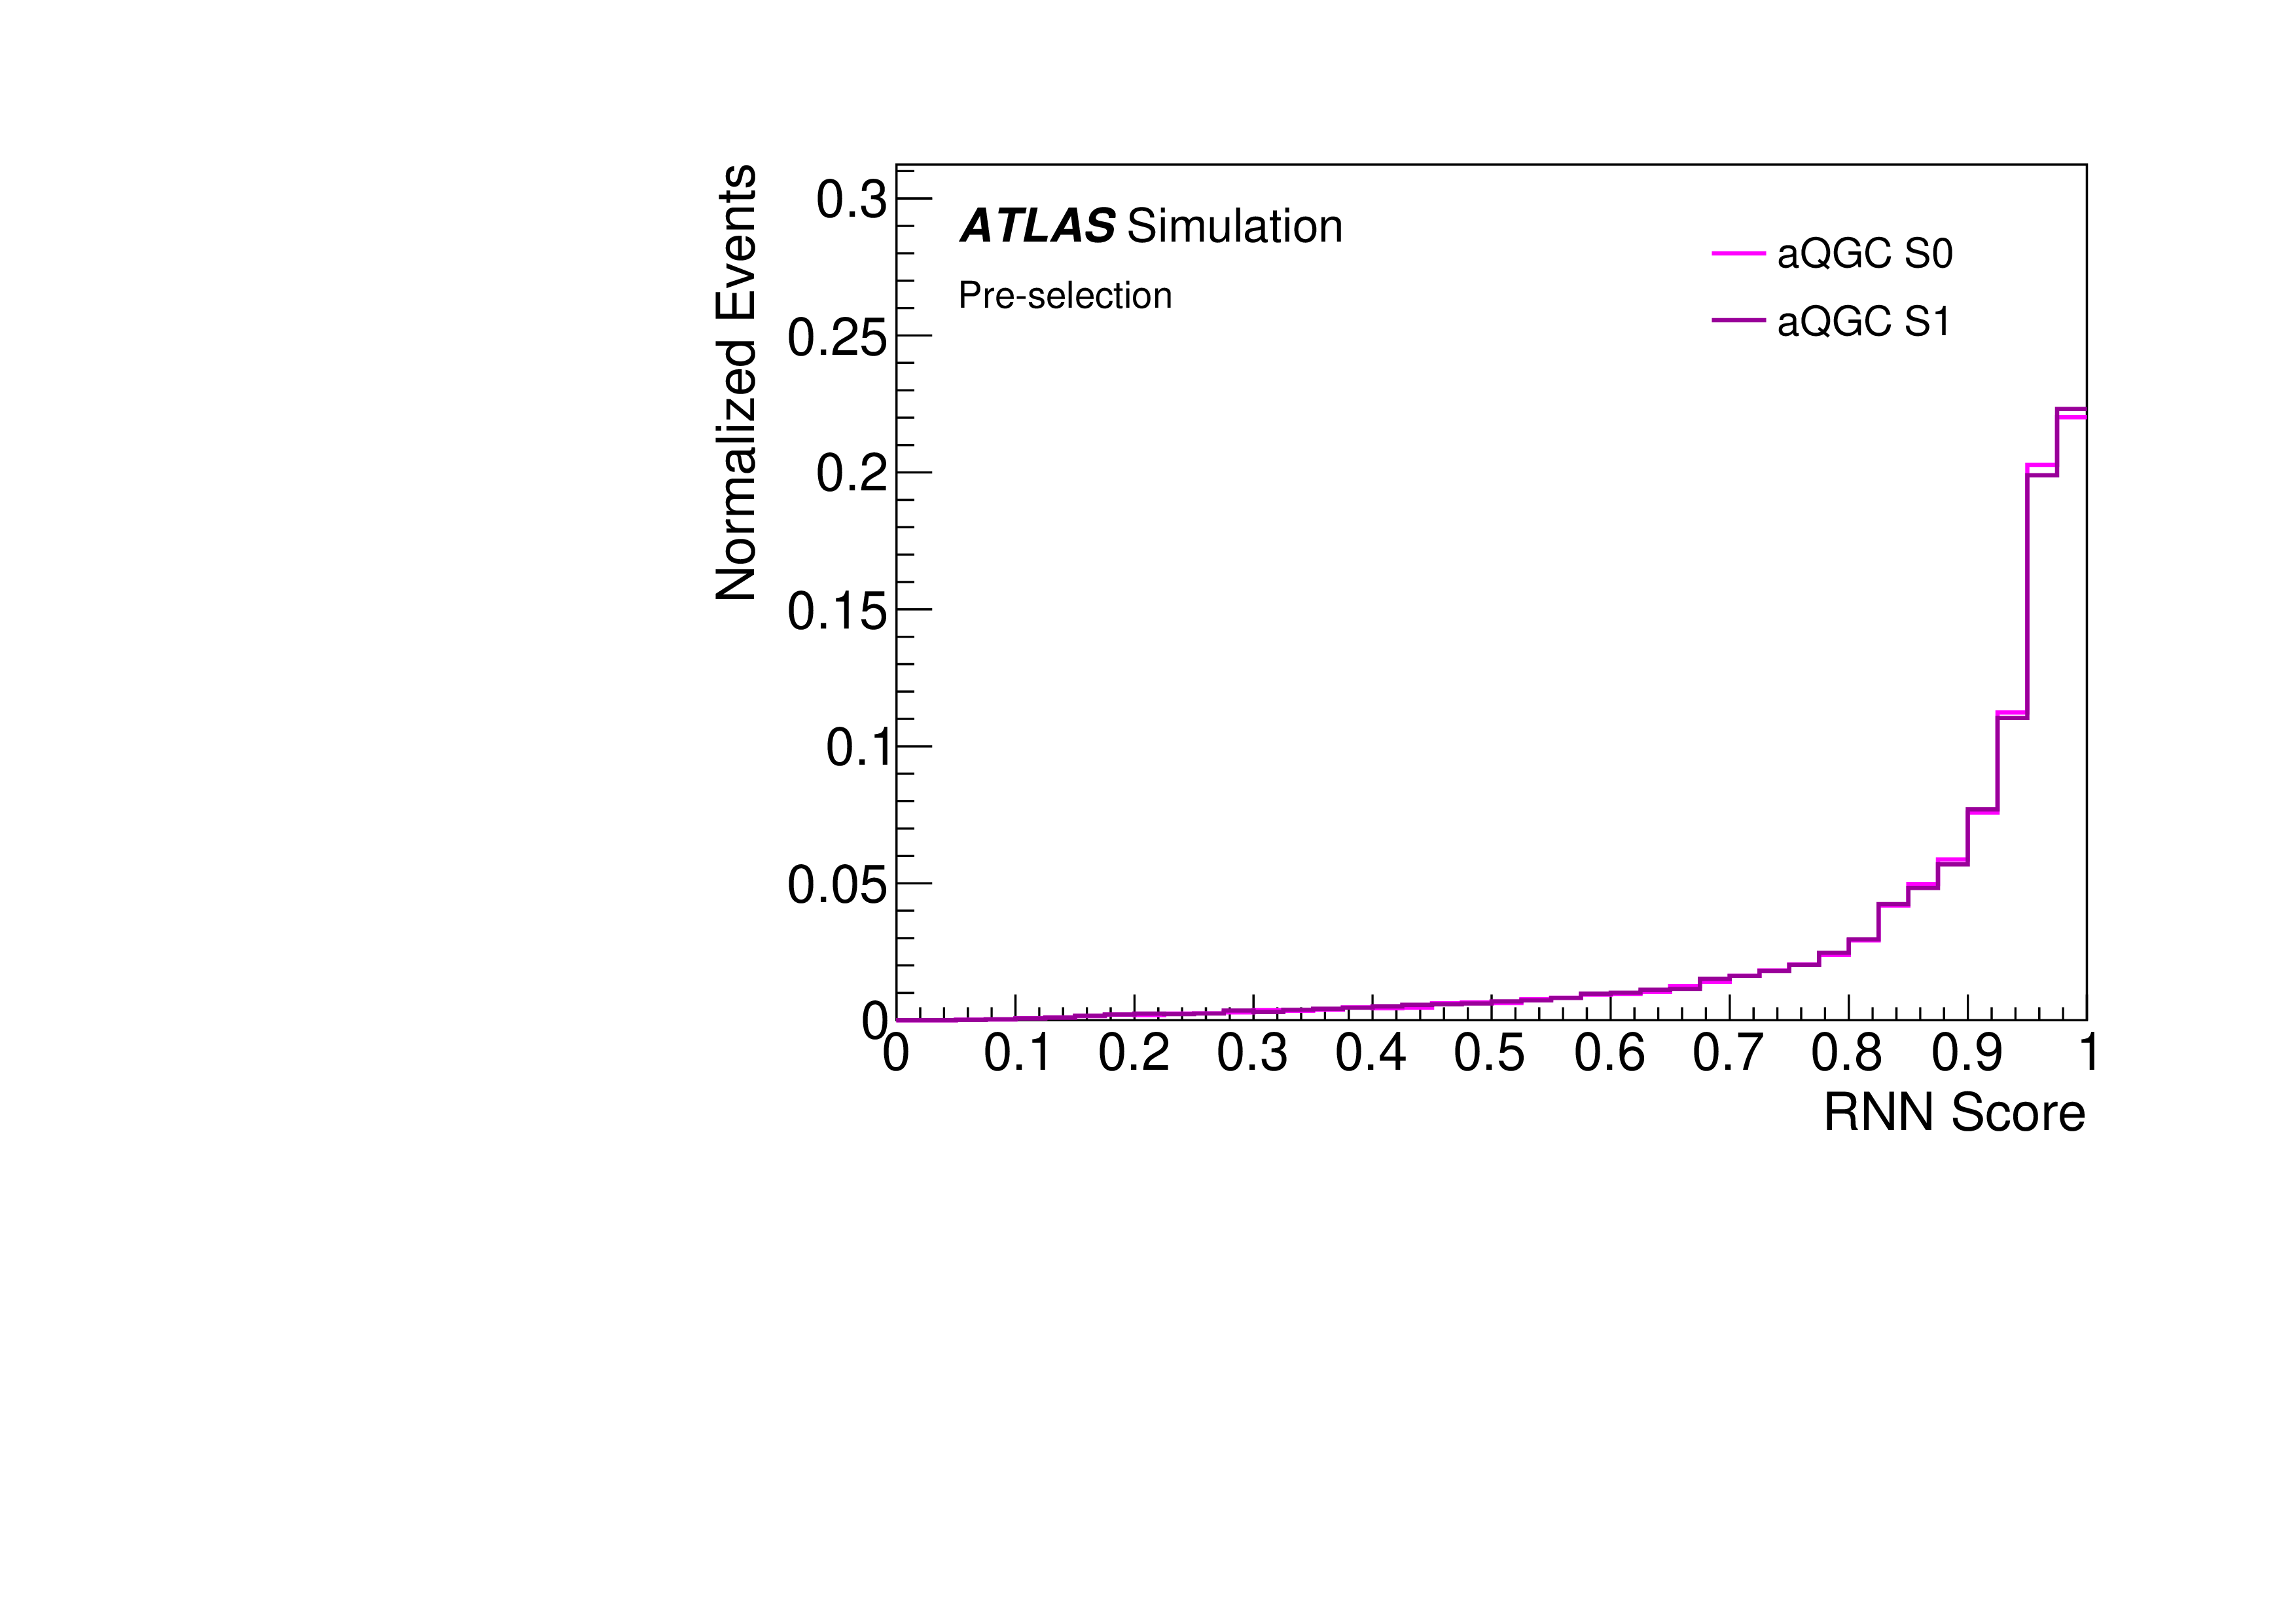
\includegraphics[width=\textwidth]{figures/vbfrnn_aqgc_v3_S.png}
\caption{Scalar}
\end{subfigure}
\begin{subfigure}[b]{0.32\textwidth}
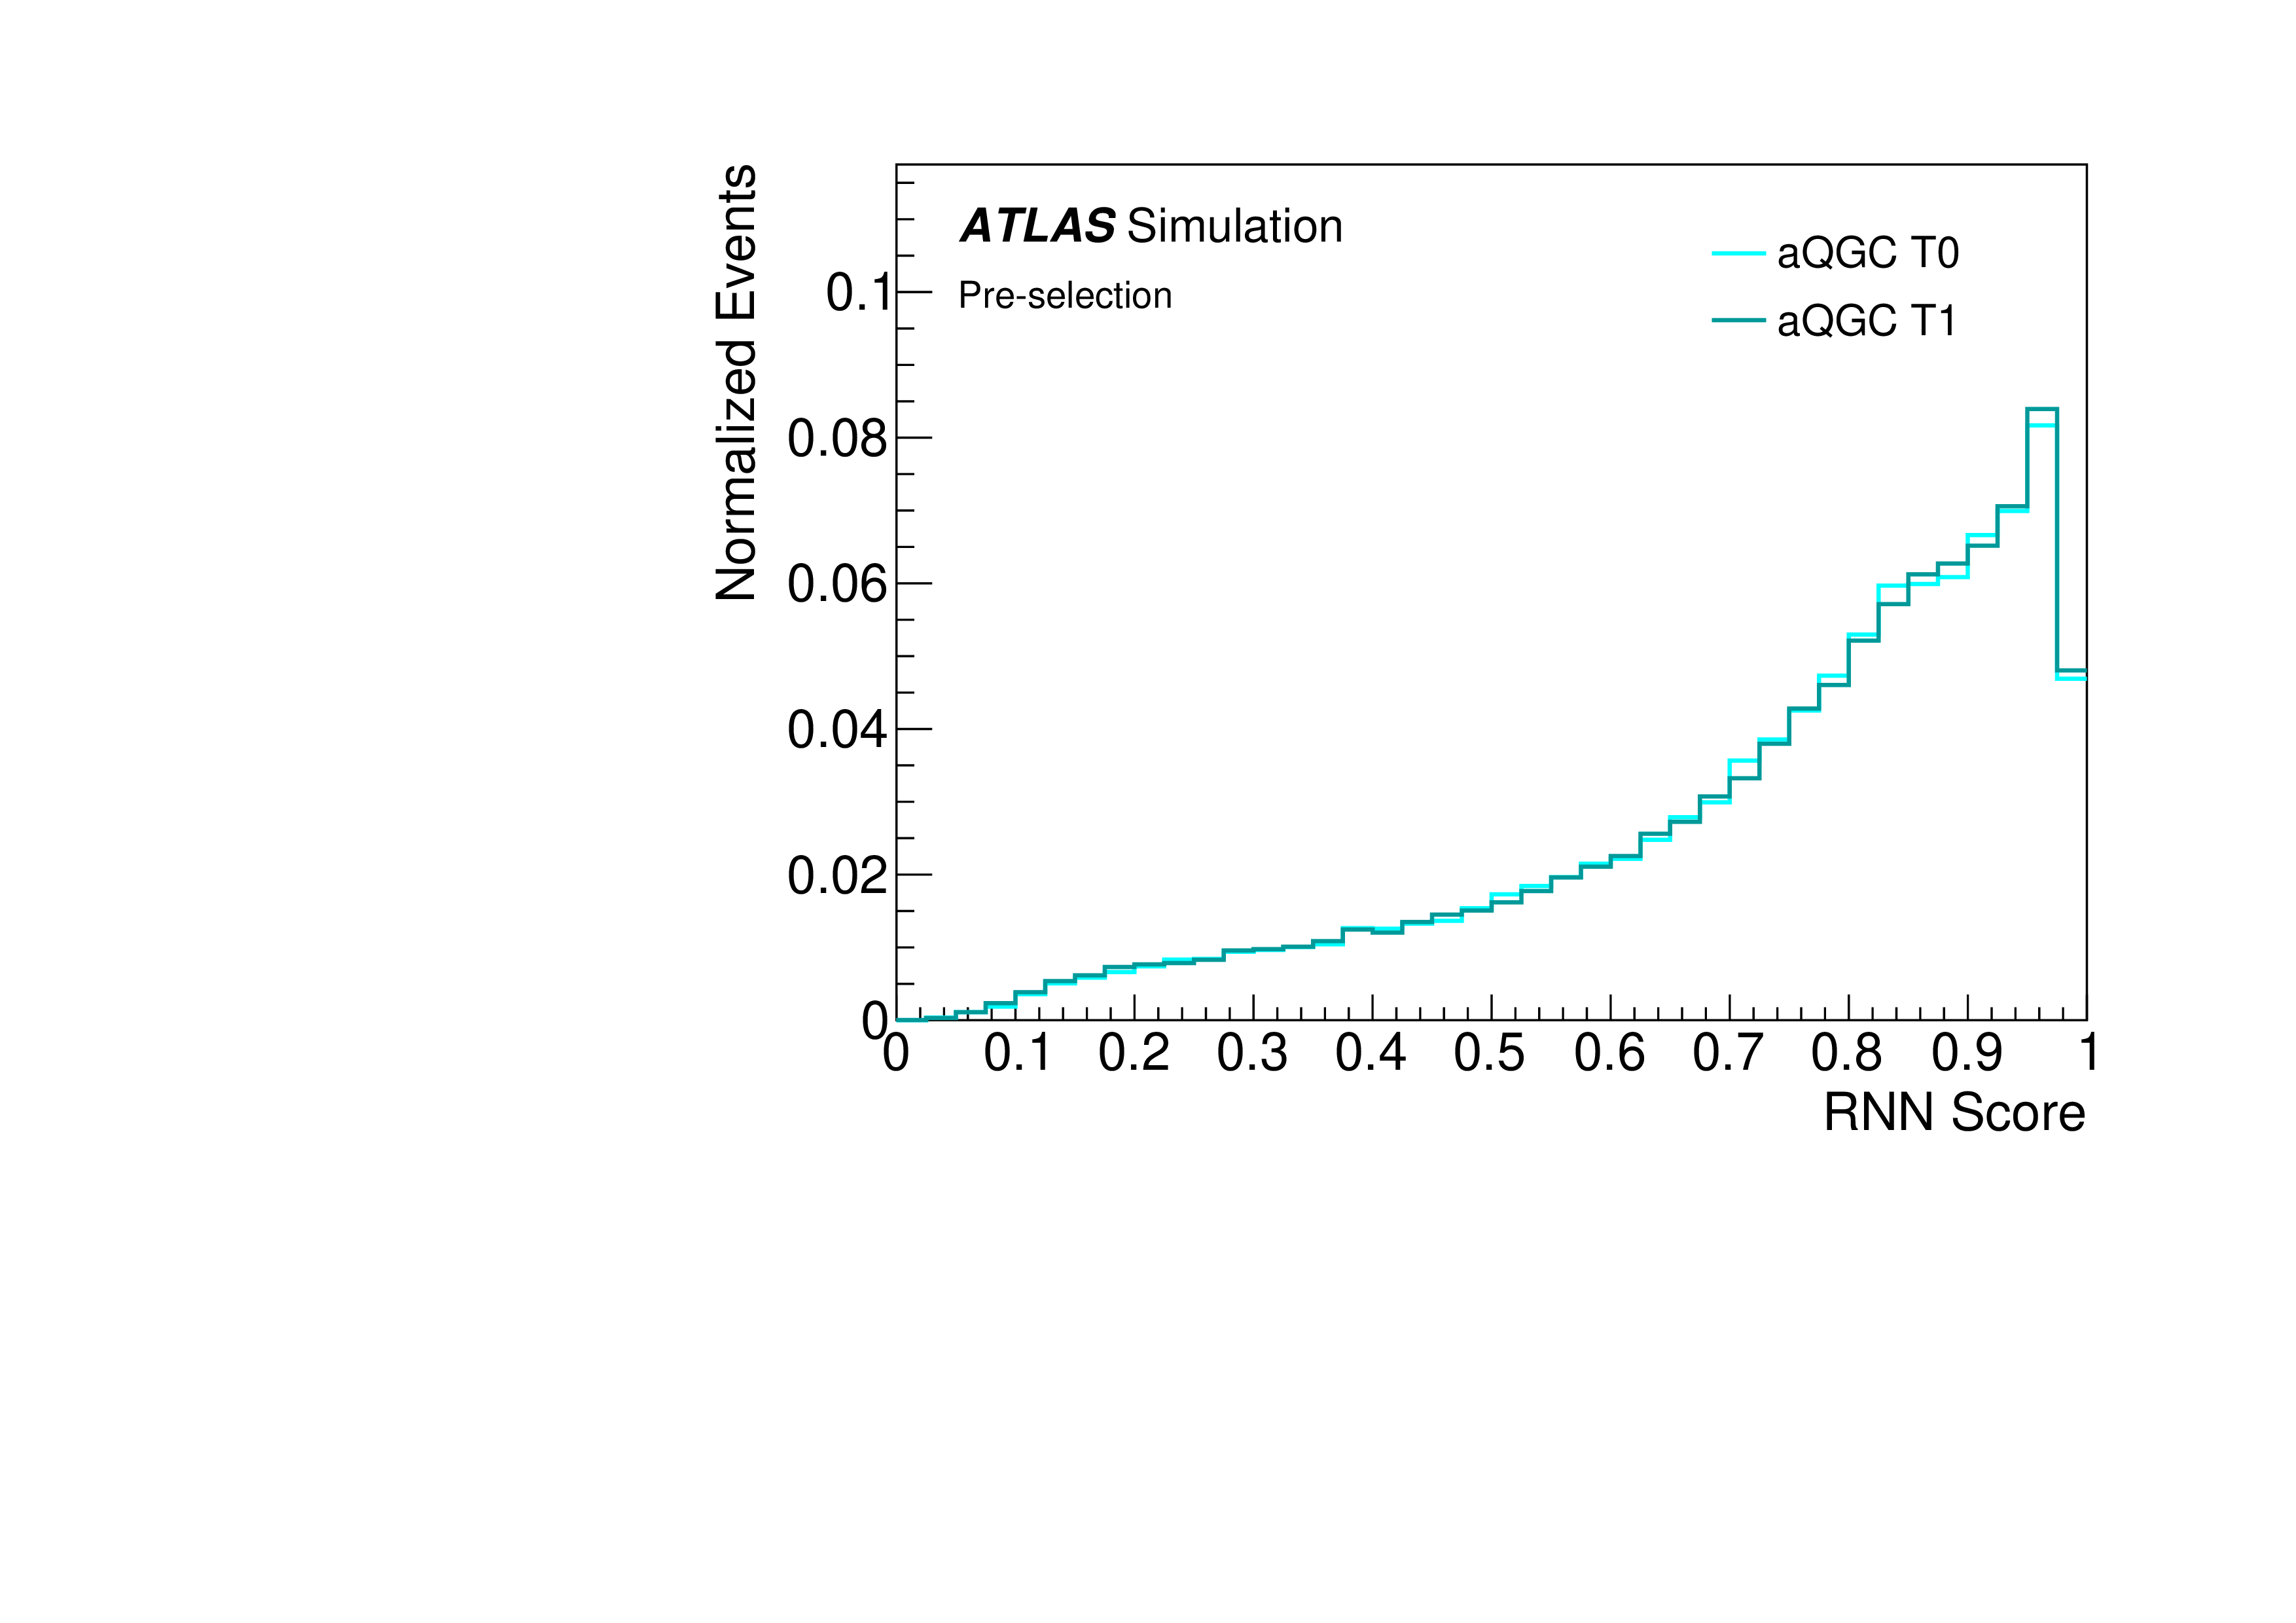
\includegraphics[width=\textwidth]{figures/vbfrnn_aqgc_v3_T.png}
\caption{Tensor}
\end{subfigure}
\begin{subfigure}[b]{0.32\textwidth}
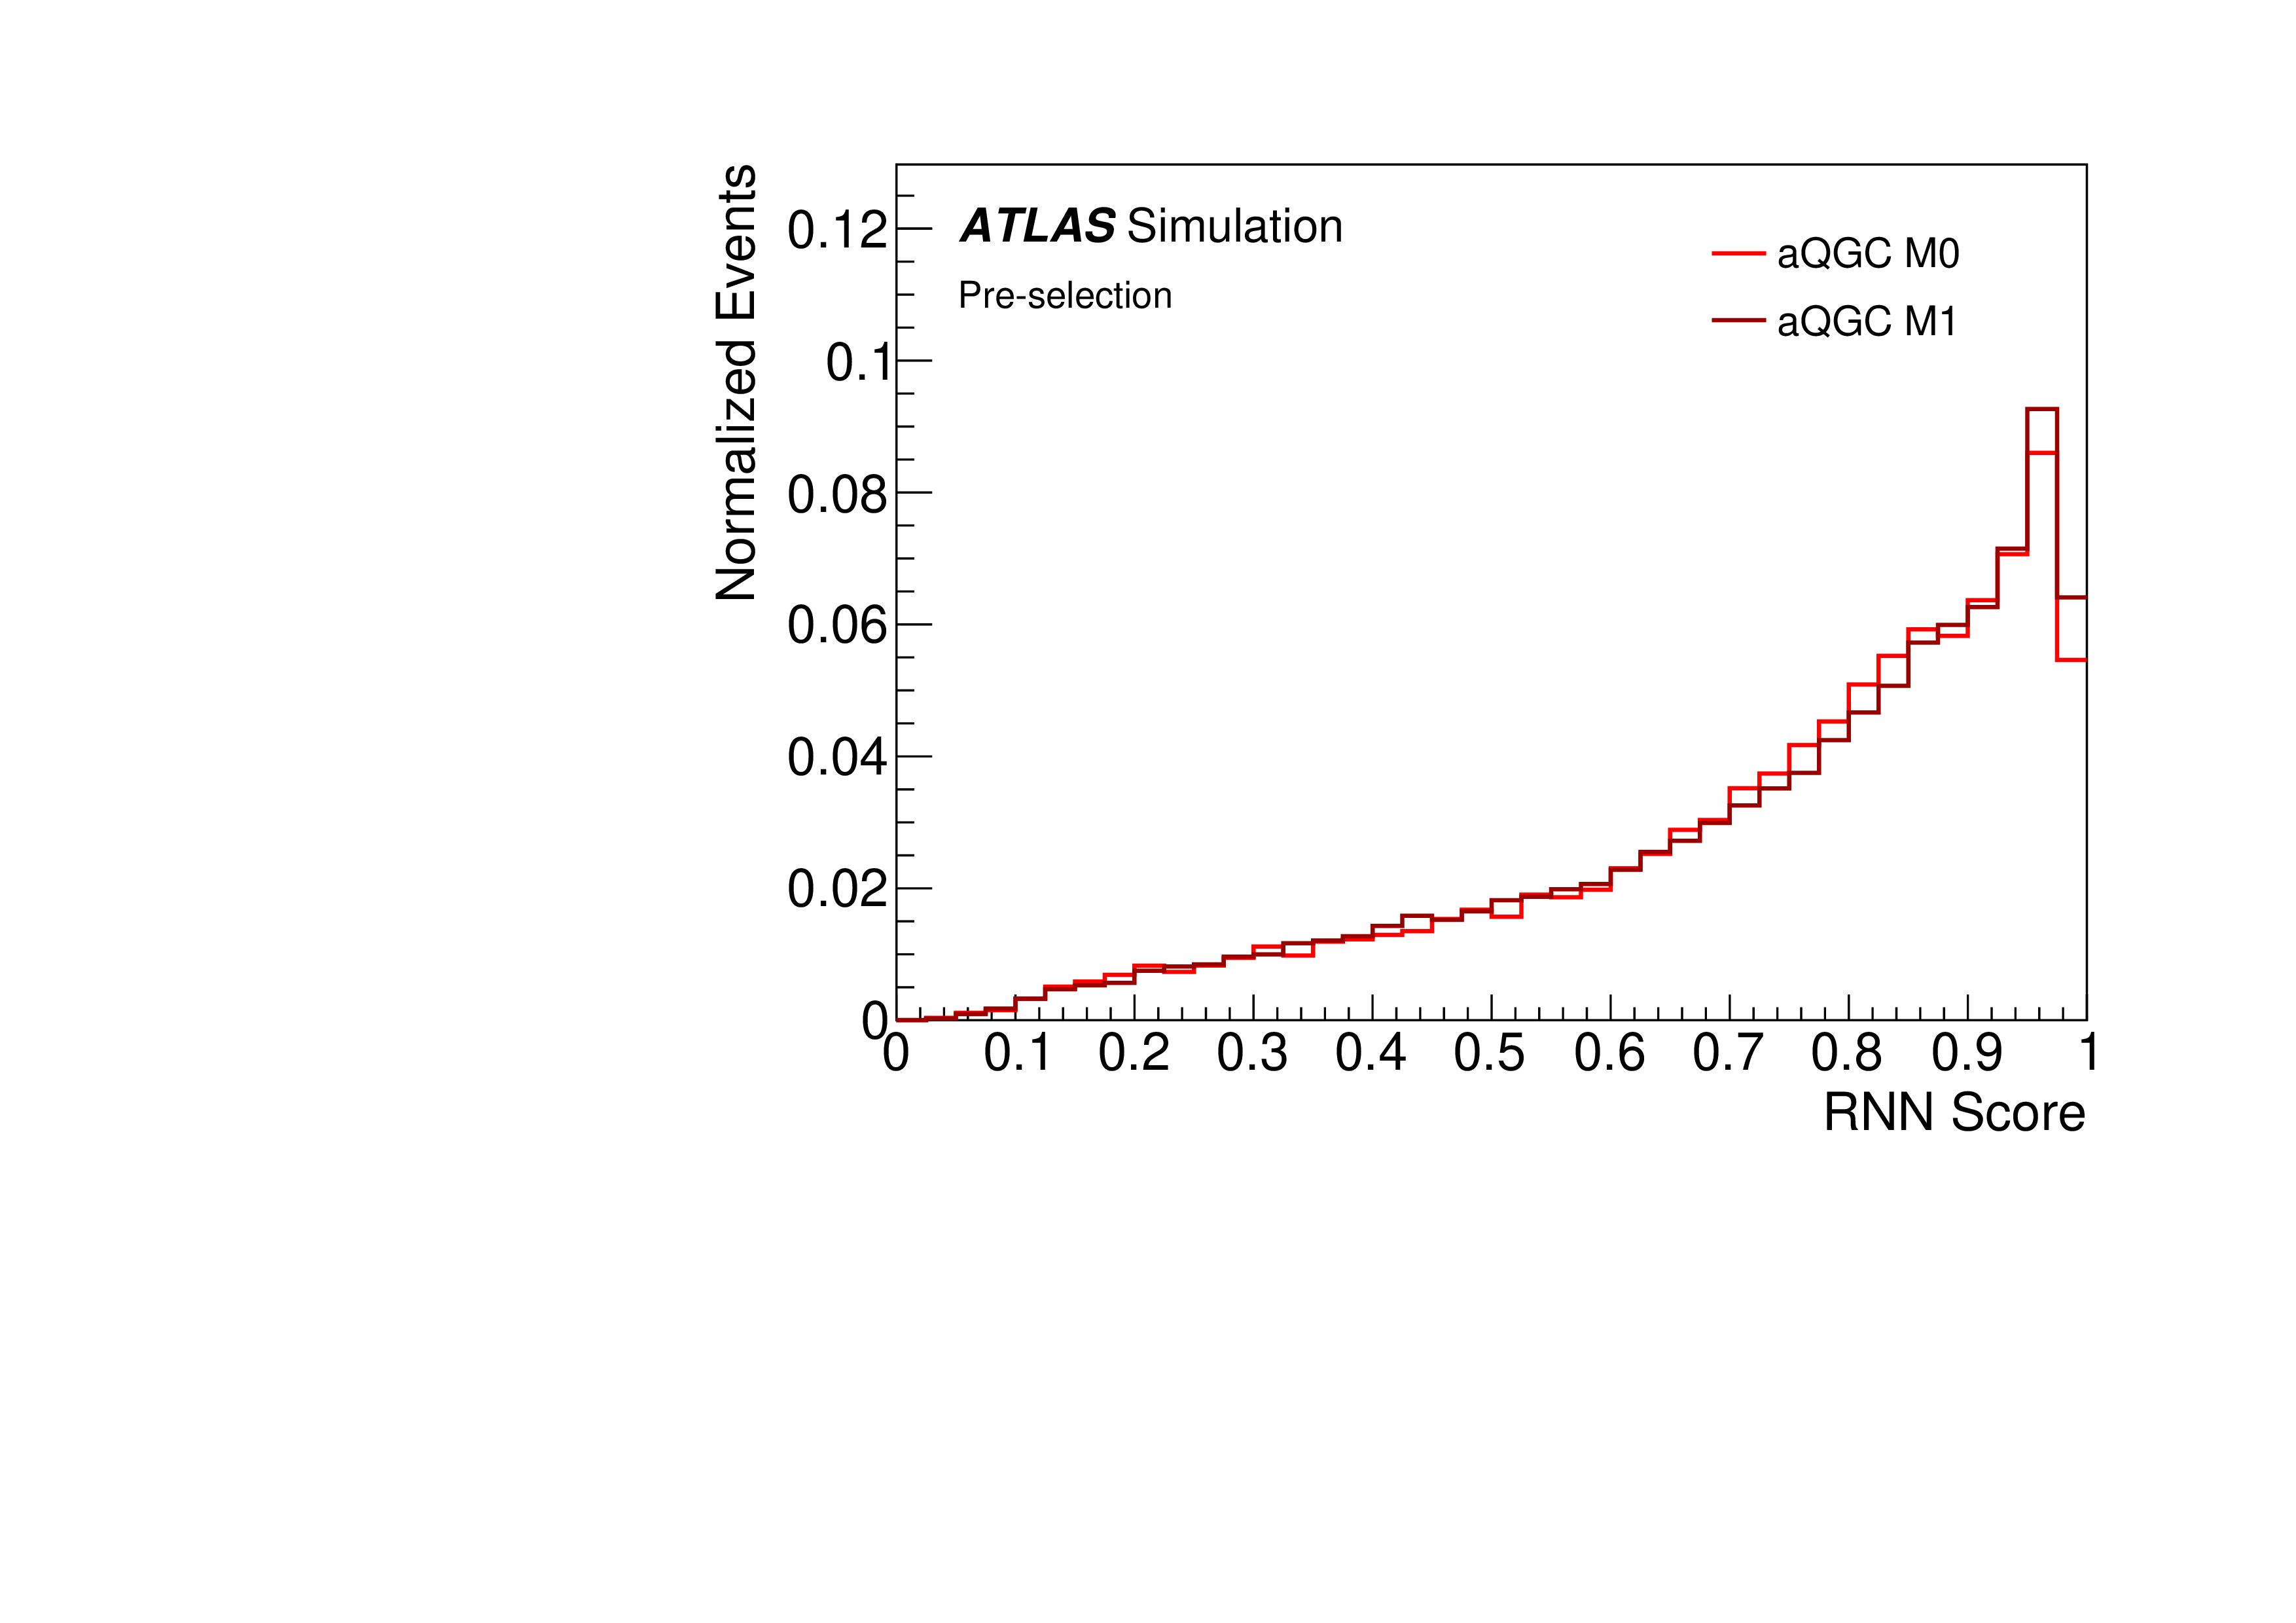
\includegraphics[width=\textwidth]{figures/vbfrnn_aqgc_v3_M.png}
\caption{Mixed}
\end{subfigure}
\caption{Normalised version~3 (6 jets, VBS vs.\ non-VBS EWK) RNN score for representative scalar, tensor and mixed aQGC operators. The response is cleanly peaked near $s\approx1$ for every operator family, confirming an operator-independent identification of the VBS topology.}
\label{fig:vbfrnn_aqgc_v3}
\end{figure}


\chapter{Sensitivity of a machine learning based aQGC discriminant}
\section{Event selection}
\section{Binary classification}
\subsection{Specialised model}
\subsection{Global model}
\section{Multi-class classification}
\section{Correlation studies}
\section{Feature ranking}
\section{Sensitivity comparison}
